\documentclass[conference]{IEEEtran}

\usepackage{cite}
\usepackage{amsmath,amssymb,amsfonts}
\usepackage{algorithmic}
\usepackage{graphicx}
\usepackage{textcomp}
\usepackage{xcolor}
\def\BibTeX{{\rm B\kern-.05em{\sc i\kern-.025em b}\kern-.08em
    T\kern-.1667em\lower.7ex\hbox{E}\kern-.125emX}}
\begin{document}

\title{Taming Complexity in Diabetes Stage Multiclass Classification: Benchmarking the Efficacy of K-Nearest Neighbors Against Optimized Regularized Logistic Regression}

\author{\IEEEauthorblockN{Gabriel Guillen}
\IEEEauthorblockA{\textit{dept. of Statistics \& Data Science} \\
\textit{University of Central Florida}\\
Orlando, United States of America \\
ga013701@ucf.edu}}


\maketitle

\begin{abstract}
This study addresses the challenge of multiclass classification in diabetes stages by benchmarking the predictive efficacy of $K$-Nearest Neighbors (KNN) against Regularized Logistic Regression. While investigating which of these contrasting modeling approaches is more competitive in simultaneously predicting a suite of diabetes-related predictors. The report details the performance of various regularization techniques (LASSO, ElasticNet, and Ridge) and evaluates model robustness, ultimately identifying the most recommendable model based on accuracy and $F_1$ score.\\
\end{abstract}

\section{\textbf{Introduction}}
\indent This study compares two fundamental classification models, \textbf{K-Nearest Neighbors} (KNN) and \textbf{Logistic Regression}, for classifying diabetes stages. Using a large dataset of over one hundred thousand observations and twenty-plus predictors, the primary goal is to determine the most effective modeling approach for complex diabetes stages classification.\\
\indent The comparison focuses specifically on evaluating the impact of different penalization techniques (such as ($\text{L}_1$) and ($\text{L}_2$) regularization) on Logistic Regression performance. Model efficacy was assessed using accuracy rates and the weighted $F_1$ metric.\\
\indent A secondary but crucial focus of this work was also on feature selection and importance. Aimed to identify the feature subset that consistently proves most influential across the compared models for accurate diabetes stage classification. \\
\indent This analysis provides an evidence-based recommendation for selecting the optimal model given the trade-off between predictive accuracy and feature interpretability. \\

\subsection{\textbf{Dataset Structure}}
\indent The dataset \cite{rakesh_kolipaka_ranjith_kumar_digutla_2025} used in this analysis comprises $100,000$ \textbf{unique patient records} ensuring privacy preservation designed for diabetes risk prediction but adapted here for classification. It features over $35$ columns encompassing diverse data types, including numeric measurements (e.g. age, BMI, glucose, HbA1c) and categorical indicators (e.g. gender, family history, smoking status).\\
\indent The target variable for this multiclass (where $N > 2$ classes exist) analysis was \textbf{diabetes stage} (disease severity), defined by the following five classes:
\begin{itemize}
	\item No Diabetes
	\item Pre-Diabetes
	\item Type 1 Diabetes
	\item Type 2 Diabetes
	\item Gestational Diabetes
\end{itemize}
\indent The dataset exhibited significant \textbf{class imbalance}. Specifically, two classes dominated the distribution: Type 2 Diabetes accounted for $60\%$ of the instances, and Pre-Diabetes accounted for $32\%$.

\section{\textbf{Methods}}

\subsection{\textbf{Data Preparation}}

\indent The initial dataset of 100,000 observations was preprocessed for the multiclass analysis, which targeted the \textbf{diabetes stage} (disease severity). Features that were not primary classification predictors, including \texttt{glucose\_fasting}, \texttt{hba1c}, \texttt{diabetes\_risk\_score}, \texttt{diagnosed\_diabetes}, \texttt{hypertension\_history}, and \texttt{cardiovascular\_history}, were excluded from the analysis.

\indent Numeric features were standardized using \textbf{Standard Scaling} to achieve a zero mean ($\mu=0$) and unit variance ($\sigma=1$). $$z = \frac{x - \mu}{\sigma}$$  This method ensures that all features contribute equally to the modeling process.\\
\indent Categorical variables (\texttt{gender}, \texttt{ethnicity}, \texttt{education level}, \texttt{income level}, \texttt{employment status}, and \texttt{smoking status}) were converted into a binary numerical format using \textbf{One-Hot Encoding} (OHE), avoiding assumptions of ordinality.\\
\indent The fully processed dataset was split into training and testing partitions using a 75\% / 25\% ratio to guarantee consistent and unbiased evaluation across all experimental models.\\

\subsection{\textbf{Classification Models Used}}

\begin{enumerate}
	\item \textbf{K-Nearest Neighbors (KNN)}: algorithm naturally extends to multiclass problems without requiring structural modification. Given an unlabeled data point, the algorithm calculates its distance to all points in the training set and identifies the $K$ closest neighbors. The data point is then assigned the class label that is most frequent among these $K$ neighbors—this is known as the \textbf{majority voting} rule.
	\item \textbf{Logistic Regression}: While intrinsically designed as a binary classifier, Logistic Regression is effectively adapted for multiclass problems through the \textbf{One-vs-Rest (OvR)} strategy. This method constructs $N$ independent binary models, where each model is specifically trained to differentiate one target class from the aggregate of all remaining classes.
\end{enumerate}

\subsection{\textbf{Tuning}}

\indent Due to computational constraints on the large dataset, resource-intensive methods like stepwise selection were omitted. \\

\subsubsection{\textbf{KNN Tuning and Feature Selection}} 

The optimal number of neighbors ($K$) for the KNN classifier was determined through a robust 5-fold cross-validation process.

\begin{table}[h]
	\centering
	\caption{Cross-Validation Performance for K-Nearest Neighbors (KNN)}
	\label{tab:knn_tuning}
	\begin{tabular}{| c | c |} % Using basic 'c' alignment and vertical lines
		\hline % Using \hline instead of \toprule
		$K$ (Tried Neighbors) & Cross-Validation weighted $F_1$  \\
		\hline % Using \hline instead of \midrule
		7 & 0.725712081 \\
		8 & 0.726563779 \\
		11 & 0.736917977 \\
		15 & 0.744016863 \\
		20 & 0.747460871 \\
		\hline % Using \hline instead of \bottomrule
	\end{tabular}
\end{table}

\indent The evaluation metric used for hyperparameter optimization was the \textbf{weighted $F_1$ score}, which is particularly suitable for multiclass and imbalanced datasets as it accounts for the precision and recall of each class.\\
\indent The results of the grid search, detailed in Table \ref{tab:knn_tuning}, indicated that the highest performance was achieved with an optimal neighbor count of $K=20$. \\

\indent Feature selection for \textbf{KNN} was implemented using the \textbf{Least Absolute Shrinkage and Selection Operator (Lasso)} regularization, which automatically selects features by driving insignificant coefficients to zero. This methodology is particularly valuable in high-dimensional datasets as it enhances model interpretability and reduces the risk of overfitting by producing a sparser model.\\

\begin{table}[htbp]
	\centering
	\caption{Features Selected by Lasso Regularization (Total $N=9$)}
	\label{tab:knn_selected_features}
	\begin{tabular}{| l |}
		\hline
		\textbf{Selected Feature Name} \\
		\hline
		\multicolumn{1}{|c|}{\textbf{Categorical Features}} \\ % Section Header
		\hline
		gender\_Female \\
		gender\_Male \\
		gender\_Other \\
		ethnicity\_Asian \\
		income\_level\_Lower-Middle \\
		employment\_status\_Student \\
		\hline
		\multicolumn{1}{|c|}{\textbf{Binary Features}} \\ % New Section Header
		\hline
		family\_history\_diabetes \\
		\hline
		\multicolumn{1}{|c|}{\textbf{Numerical Features}} \\ % Section Header
		\hline
		age \\
		glucose\_postprandial \\
		\hline
	\end{tabular}
\end{table}

\indent The resulting subset of features in Table \ref{tab:knn_selected_features}, identified by non-zero coefficients, was then used as the input space for the KNN algorithm, leading to a more robust and computationally efficient classifier.\\

\subsubsection{\textbf{Logistic Regression Tuning}}
For the Logistic Regression models, a comprehensive regularization comparison was performed using three penalties across separate models: \textbf{\text{$\text{L}_1$} (Lasso)}, \textbf{\text{$\text{L}_2$} (Ridge)}, and \textbf{ElasticNet}, to evaluate their impact on generalization and feature parsimony for the multiclass problem.\\
\indent \textbf{Logistic/$\text{L}_1$ Model}: \textbf{Logistic Regression} combined with a \textbf{Lasso ($\text{L}_1$)} penalization yielded the most aggressive feature selection result. This approach retained only a single feature: \texttt{glucose\_postprandial}. \\
\indent The optimal value for the inverse Lasso tuning parameter ($C$) was determined through a 5-fold cross-validation procedure, testing values in the set $\{0.001, 0.01, 1\}$. The best-performing parameter was $C = 0.01$, chosen by optimizing the \textbf{weighted  $F_1$-score} as the primary scoring metric.\\
\indent \textbf{Logistic/$\text{L}_2$ Model}: The application of \textbf{Logistic Regression} with a \textbf{Ridge ($\text{L}_2$)} penalization resulted in a less aggressive form of regularization compared to other approaches. The optimal value for the inverse of the regularization strength ($\mathbf{C}$) was determined via a 5-fold cross-validation procedure. The search space for $C$ included ten logarithmically spaced values, specifically:
$$
C \in \{10^{-4}, 7.74 \cdot 10^{-4}, 5.99 \cdot 10^{-3}, 4.64 \cdot 10^{-2},$$
$$ 3.59 \cdot 10^{-1}, 2.78, 21.54, 166.81, 1291.55, 10000\}
$$
\indent The winning parameter was identified as $\mathbf{C = 21.54}$, which was chosen by optimizing the \textbf{weighted  $F_1$-score} as the primary scoring metric.\\
\indent \textbf{Logistic/ElasticNet Model}: The application of \textbf{Logistic Regression} with \textbf{Elastic Net} penalization adopted a tuning strategy similar to the $\text{L}_2$ (Ridge) approach, but required the optimization of two hyperparameters. The best-performing parameters were found to be $\mathbf{C = 1291.54}$ (the inverse of regularization strength) and an $\mathbf{\ell_1 \text{ ratio} = 0.34}$. This $\ell_1$ ratio specifies the balance between the $\text{L}_1$ (Lasso) and $\text{L}_2$ components of the penalty, indicating a mix of $34\%$ $\text{L}_1$ and $66\%$ $\text{L}_2$ regularization.\\

\section{\textbf{Results}}
 
\subsection{\textbf{KNN Results}}

\begin{figure}[htbp]
	\centerline{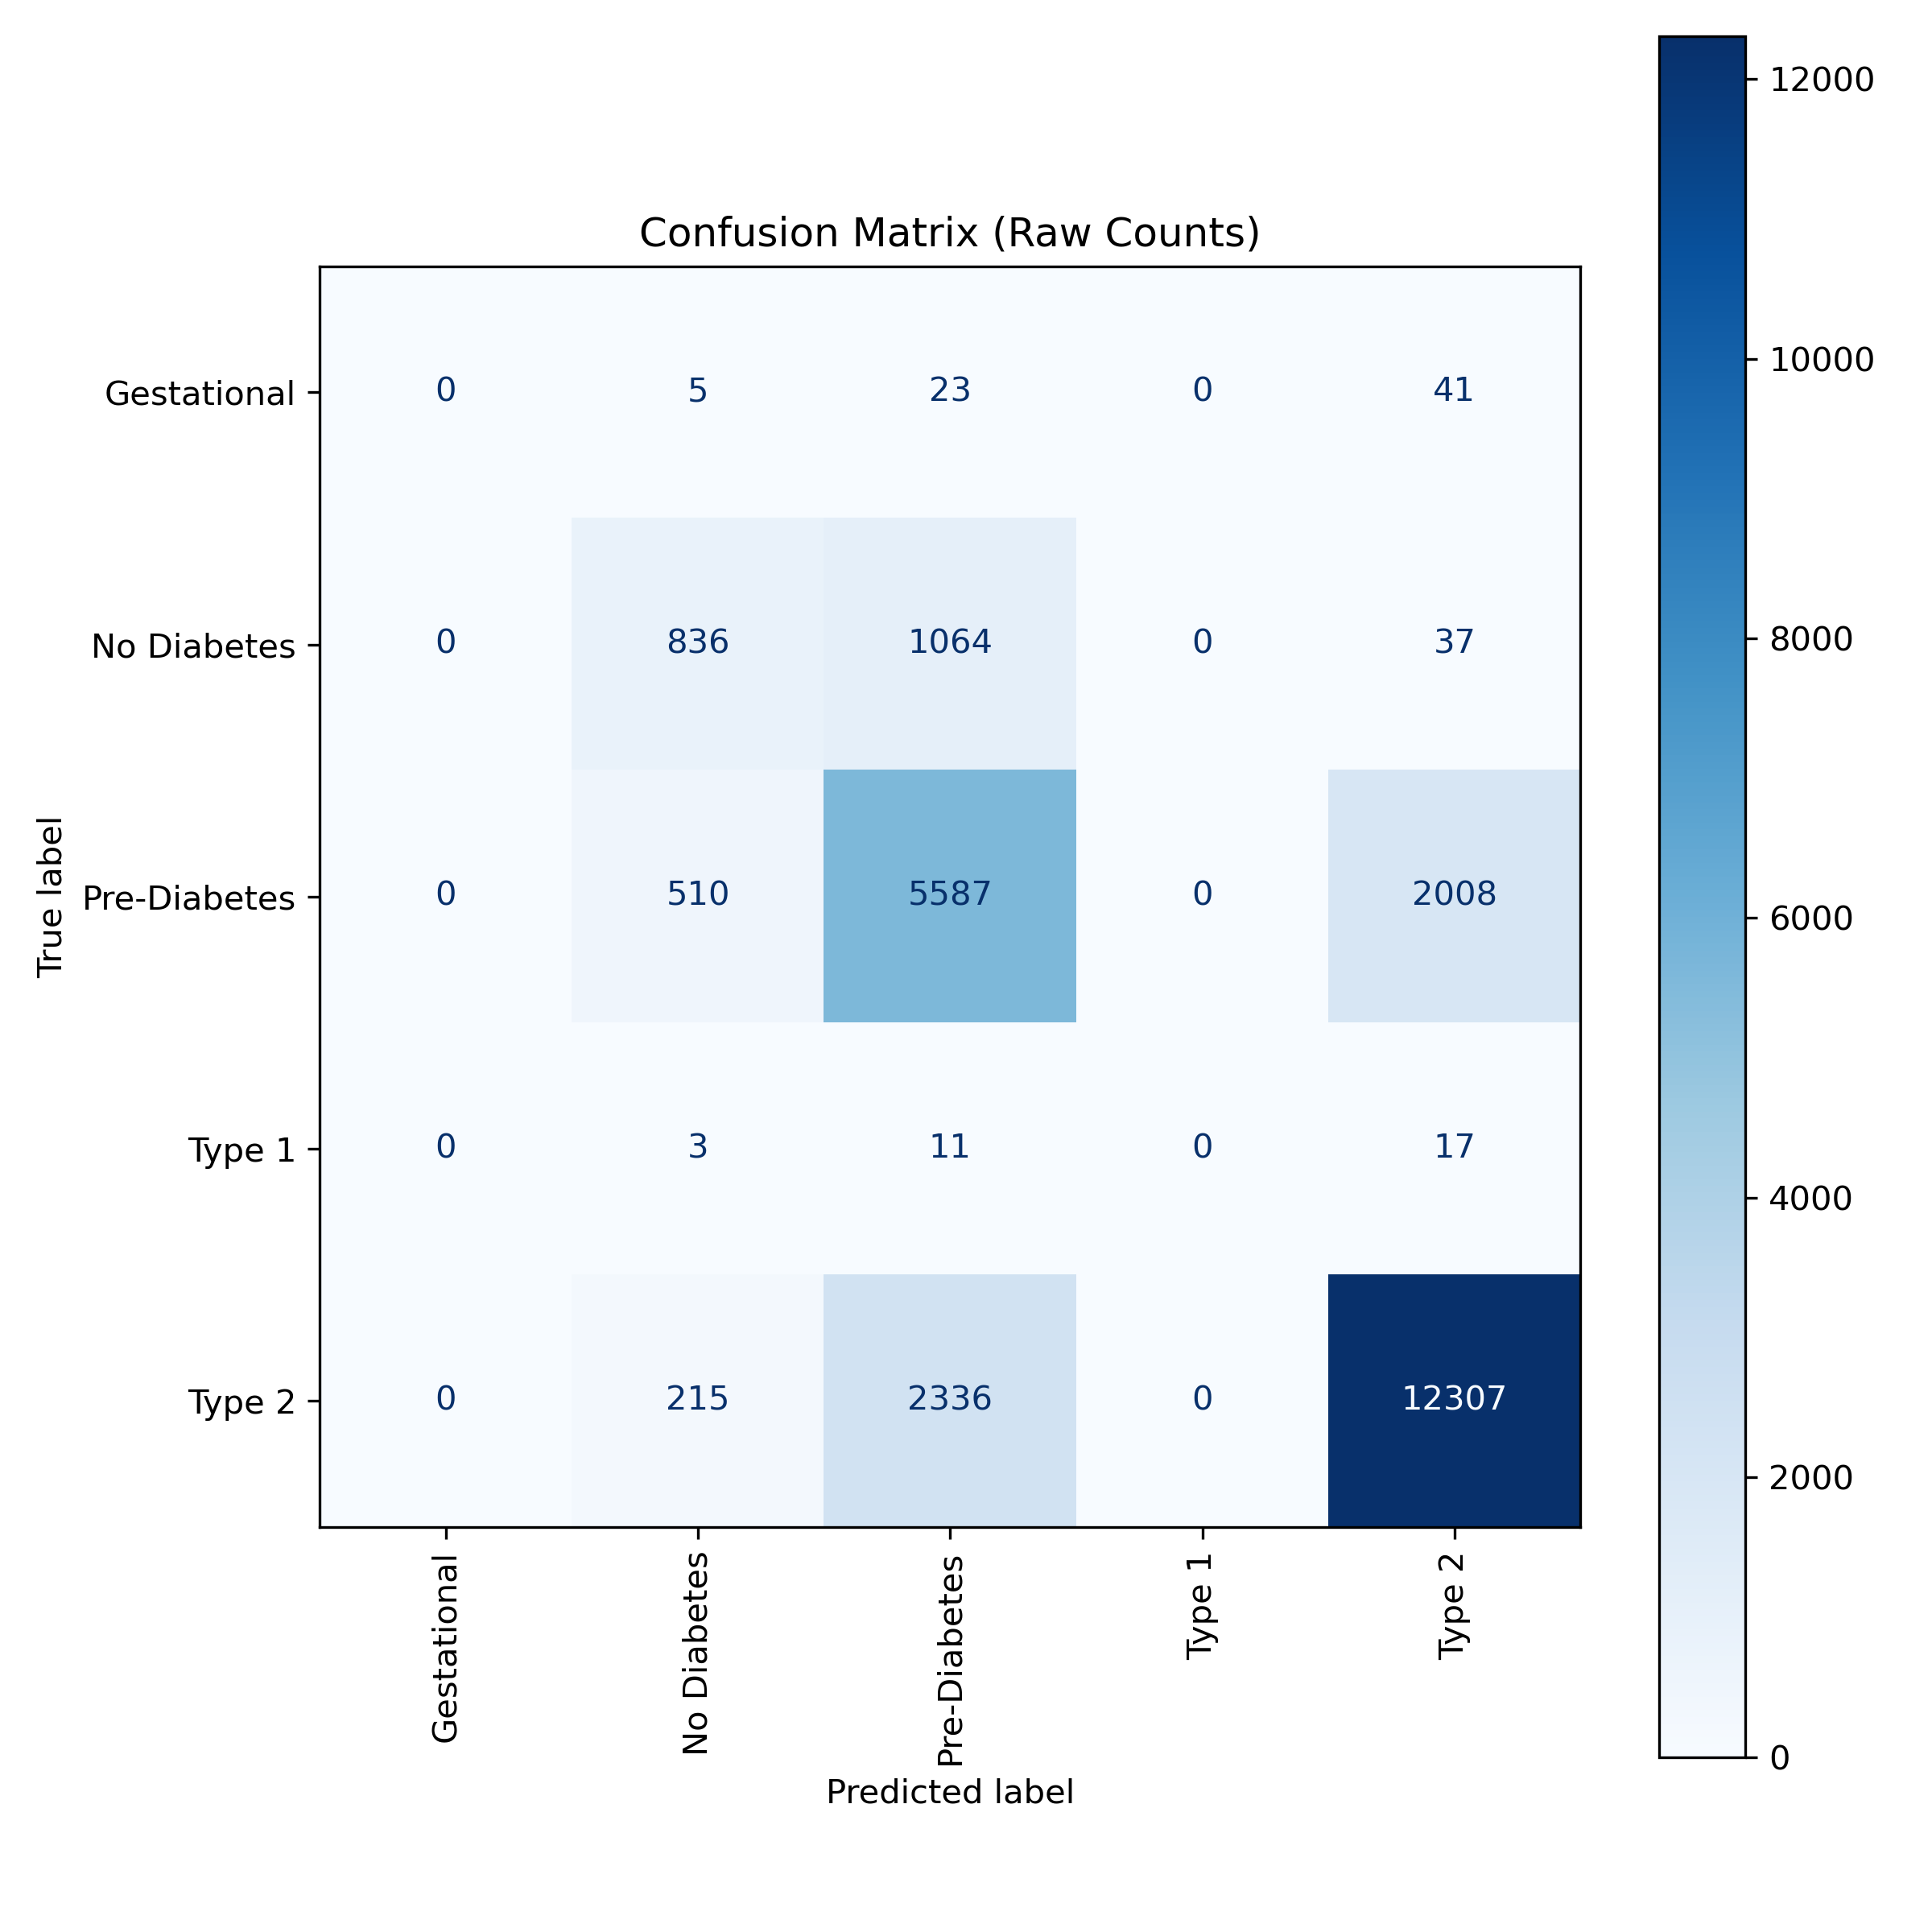
\includegraphics[scale=0.45]{knn_multiclass_confusion_matrix.png}}
	\caption{\textbf{KNN} Confusion Matrix}
	\label{knn_confusion_matrix}
\end{figure}
\subsubsection{KNN Confusion Matrix}  As shown in Figure \ref{knn_confusion_matrix}, the overall performance of the model reveals significant misclassification patterns across several classes. Most notably, \textbf{Gestational Diabetes} ($\mathbf{69}$ true cases) and \textbf{Type 1 Diabetes} ($\mathbf{31}$ true cases) were \textbf{completely misclassified}, with the majority of these cases being incorrectly labeled as \textbf{Type 2 Diabetes} ($41$ and $17$ cases, respectively), suggesting these rarer classes are severely underrepresented or highly confused with the dominant Type 2 group.\\
\indent Furthermore, the model exhibited large errors between the major classes: $\mathbf{1,064}$ true \textbf{No Diabetes} cases were misclassified as \textbf{Pre-Diabetes} (a significant Type I error), while $\mathbf{2,008}$ true \textbf{Pre-Diabetes} cases were misclassified as \textbf{Type 2} (suggesting an over-eagerness to assign the 'Type 2' label). 

\begin{figure}[htbp]
	\centerline{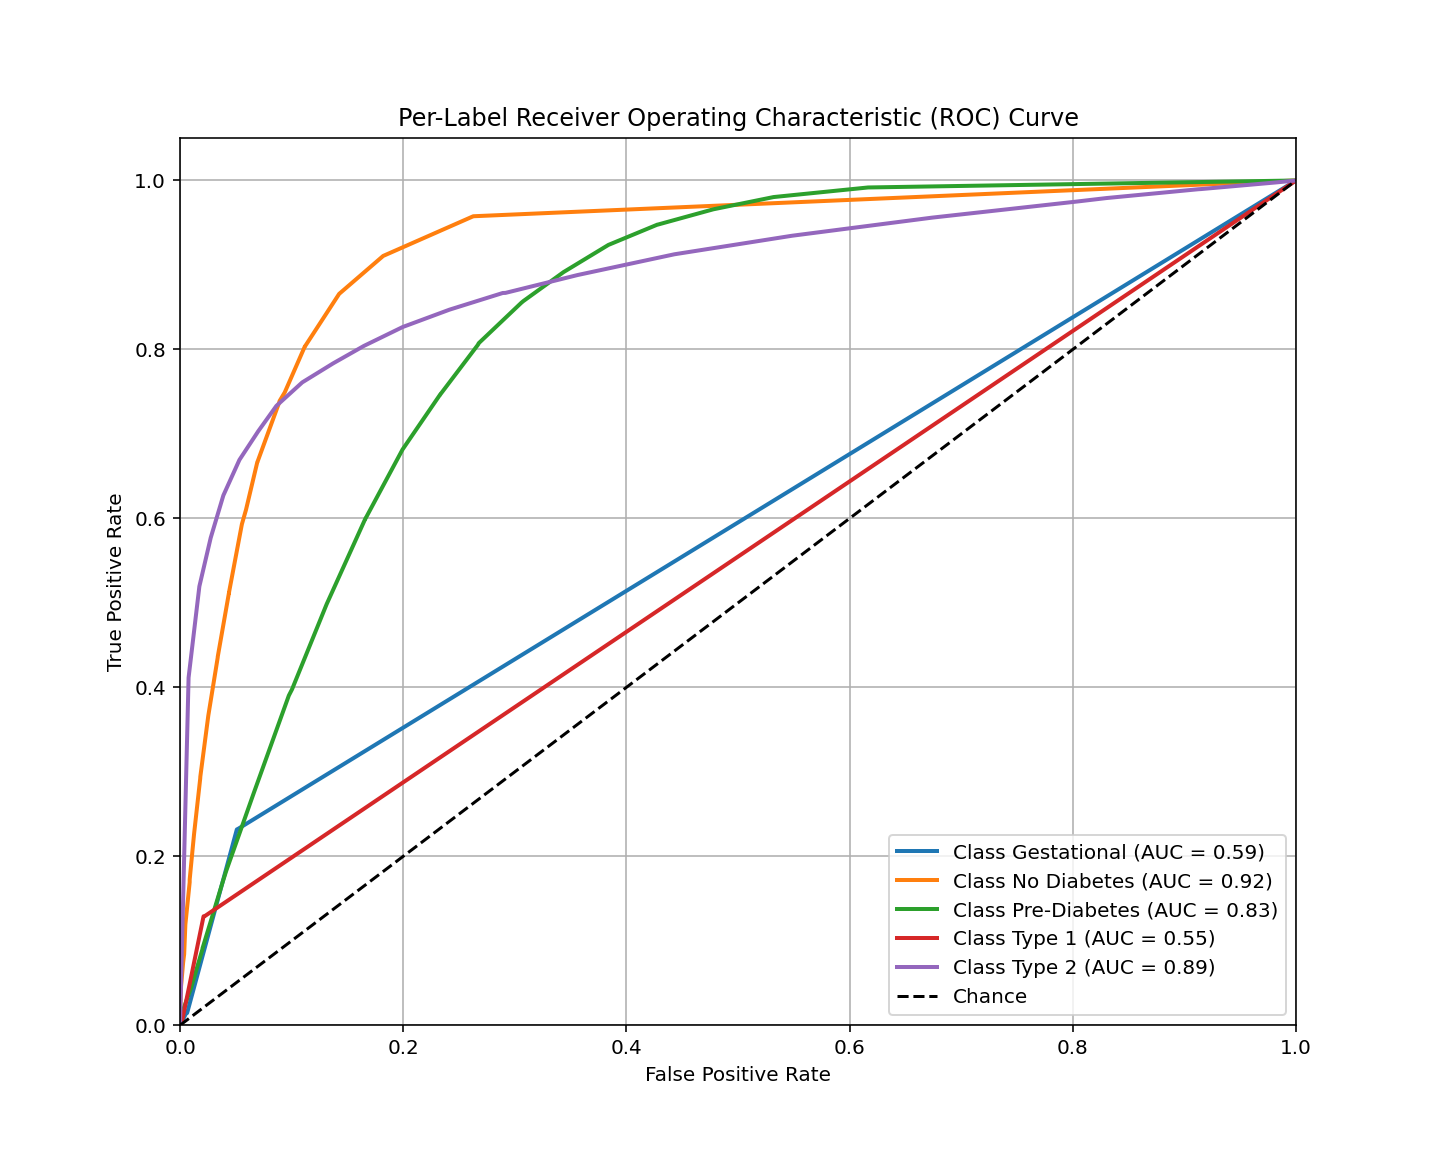
\includegraphics[scale=0.35]{knn_roc_curve.png}}
	\caption{\textbf{KNN} ROC Curve}
	\label{knn_roc_curve}
\end{figure}

\subsubsection{KNN ROC Curve} The \textbf{Receiver Operating Characteristic (ROC) curves} Figure \ref{knn_roc_curve} for the \textbf{KNN} model echo the patterns observed in the confusion matrix. The model demonstrates \textbf{excellent to very good} discriminative performance for the two most prevalent classes, achieving an \textbf{Area Under the Curve (AUC)} of $0.92$ for the \textbf{No Diabetes} class---indicating it is best at distinguishing this class---and an \textbf{AUC of $0.89$} for the \textbf{Type 2 Diabetes} class.\\ 
\indent Performance remains \textbf{solid} for the \textbf{Pre-Diabetes} class with an \textbf{AUC of $0.83$}. However, the model exhibits \textbf{poor to very poor} performance for the rarer classes, with the \textbf{Gestational Diabetes} class yielding an \textbf{AUC of $0.59$} (barely above random chance) and the \textbf{Type 1 Diabetes} class showing the weakest result with an \textbf{AUC of $0.55$}, signifying a significant struggle to correctly classify these specific distinctions.

\subsection{\textbf{Logistic Regression with  $\text{L}_1$ Results}}

\begin{figure}[htbp]
	\centerline{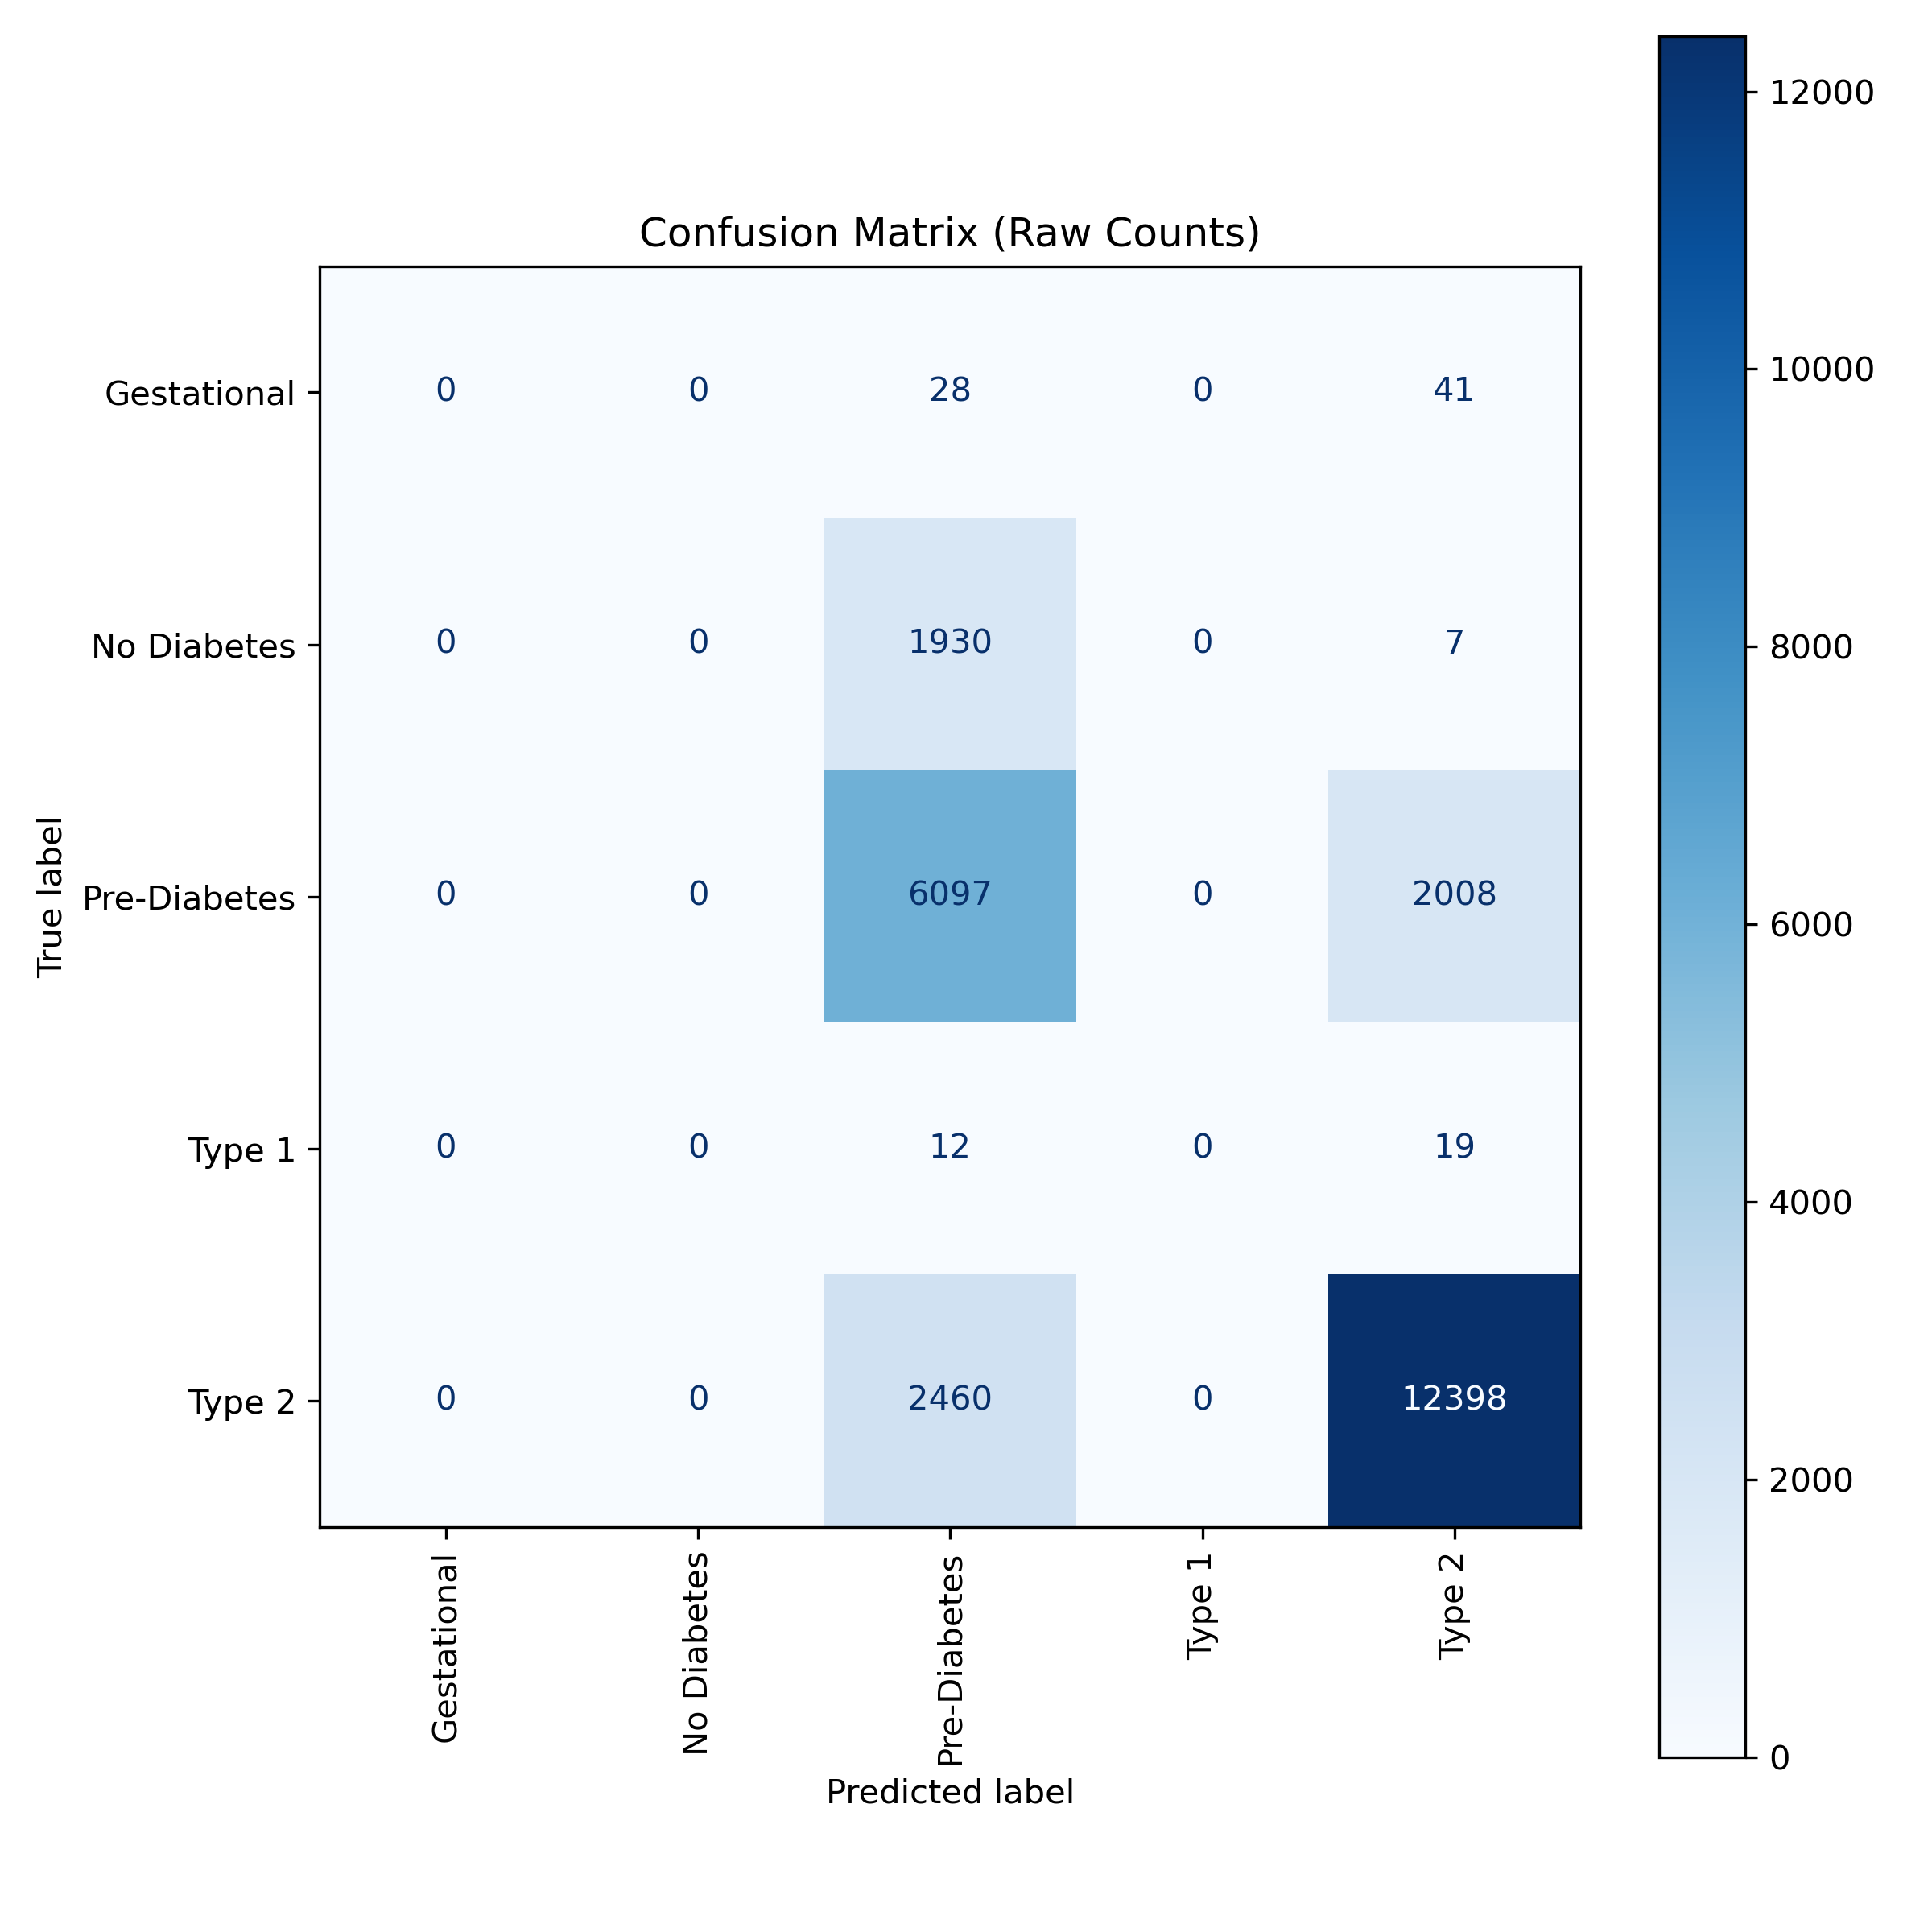
\includegraphics[scale=0.45]{log_lasso_confusion_matrix.png}}
	\caption{\textbf{Logistic/$\text{L}_1$ } Confusion Matrix}
	\label{lasso_confusion_matrix}
\end{figure}

\subsubsection{Logistic/$\text{L}_1$ Confusion Matrix} The model demonstrates a significant bias in Figure \ref{lasso_confusion_matrix} , performing well only on the \textbf{Type 2} class ($\mathbf{12,398}$ true positives) while being heavily skewed toward predicting either Pre-Diabetes or Type 2, entirely missing the Gestational, No Diabetes, and Type 1 categories, which are never correctly predicted. Specifically, all $\mathbf{69}$ actual \textbf{Gestational} cases were misclassified ($41$ as Type 2, $28$ as Pre-Diabetes), and none of the $\mathbf{31}$ actual \textbf{Type 1} cases were correctly identified ($19$ predicted as Type 2, $12$ as Pre-Diabetes). \\
\indent Furthermore, the model showed a critical failure in distinguishing non-diabetic individuals, as almost all $\mathbf{1,937}$ actual \textbf{No Diabetes} cases were incorrectly labeled as Pre-Diabetes ($\mathbf{1,930}$). While \textbf{Pre-Diabetes} had the second-highest accuracy ($\mathbf{6,097}$ true positives), there is significant confusion between the two predicted classes, with $\mathbf{2,008}$ actual Pre-Diabetes cases mistakenly called Type 2, and $\mathbf{2,460}$ actual Type 2 cases mistakenly called Pre-Diabetes. 

\begin{figure}[htbp]
	\centerline{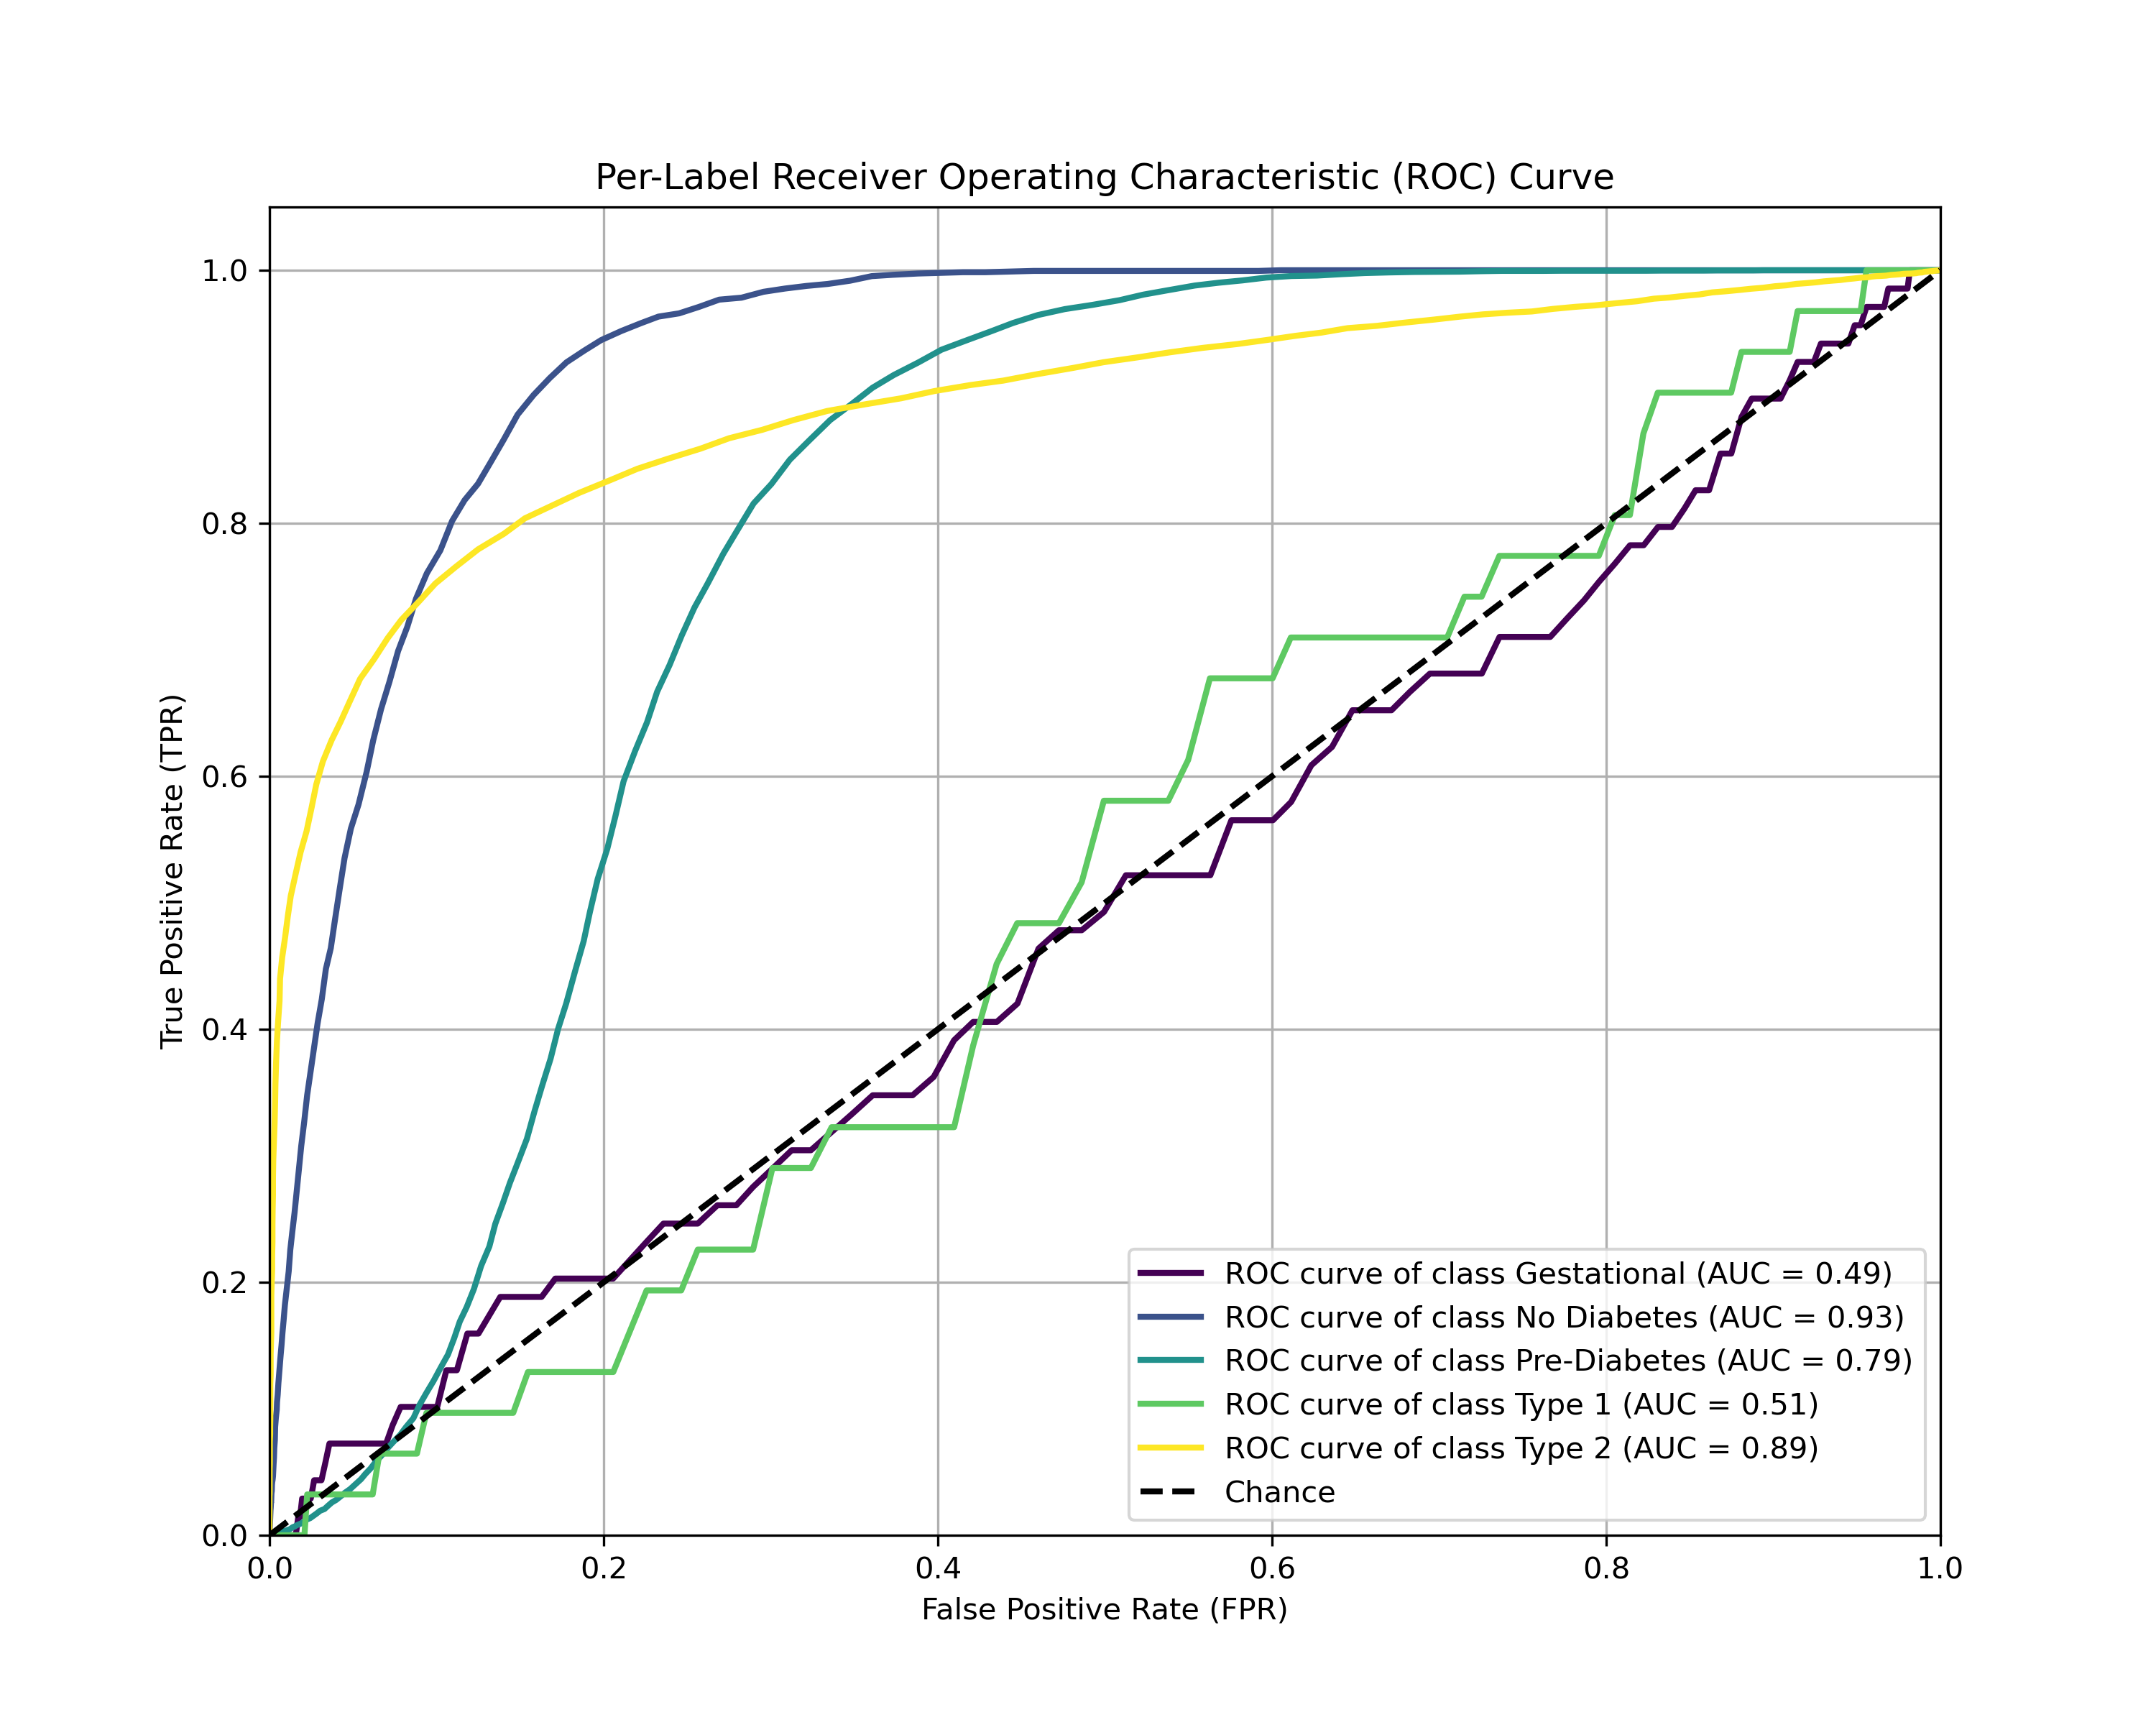
\includegraphics[scale=0.35]{log_lasso_roc_curve.png}}
	\caption{\textbf{Logistic/$\text{L}_1$ } ROC Curve}
	\label{lasso_roc_curve}
\end{figure}


\subsubsection{Logistic/$\text{L}_1$ ROC Curve} In Figure \ref{lasso_confusion_matrix} the classification model demonstrates highly varied performance across the different diabetes classes based on the ROC analysis. The \textbf{No Diabetes} class, represented by the dark blue curve, achieves an \textbf{Excellent AUC of $0.93$}, indicating high effectiveness in distinguishing it from other classes.\\ \indent This is followed closely by \textbf{Type 2} (yellow curve) with a \textbf{Very Good AUC of $0.89$}. Performance remains \textbf{Good/Acceptable} for \textbf{Pre-Diabetes} (teal/medium blue curve) with an \textbf{AUC of $0.79$}. However, the model performs \textbf{Poorly/Near Chance} for \textbf{Type 1} (light green curve), with an AUC of only $0.51$, suggesting a significant struggle. Performance is even worse for \textbf{Gestational} (purple/black curve) with an \textbf{AUC of $0.49$}, which is considered worse than random guessing, implying systematic prediction errors for this specific class.\\

\subsection{\textbf{Logistic Regression with  $\text{L}_2$ Results}}

\begin{figure}[htbp]
	\centerline{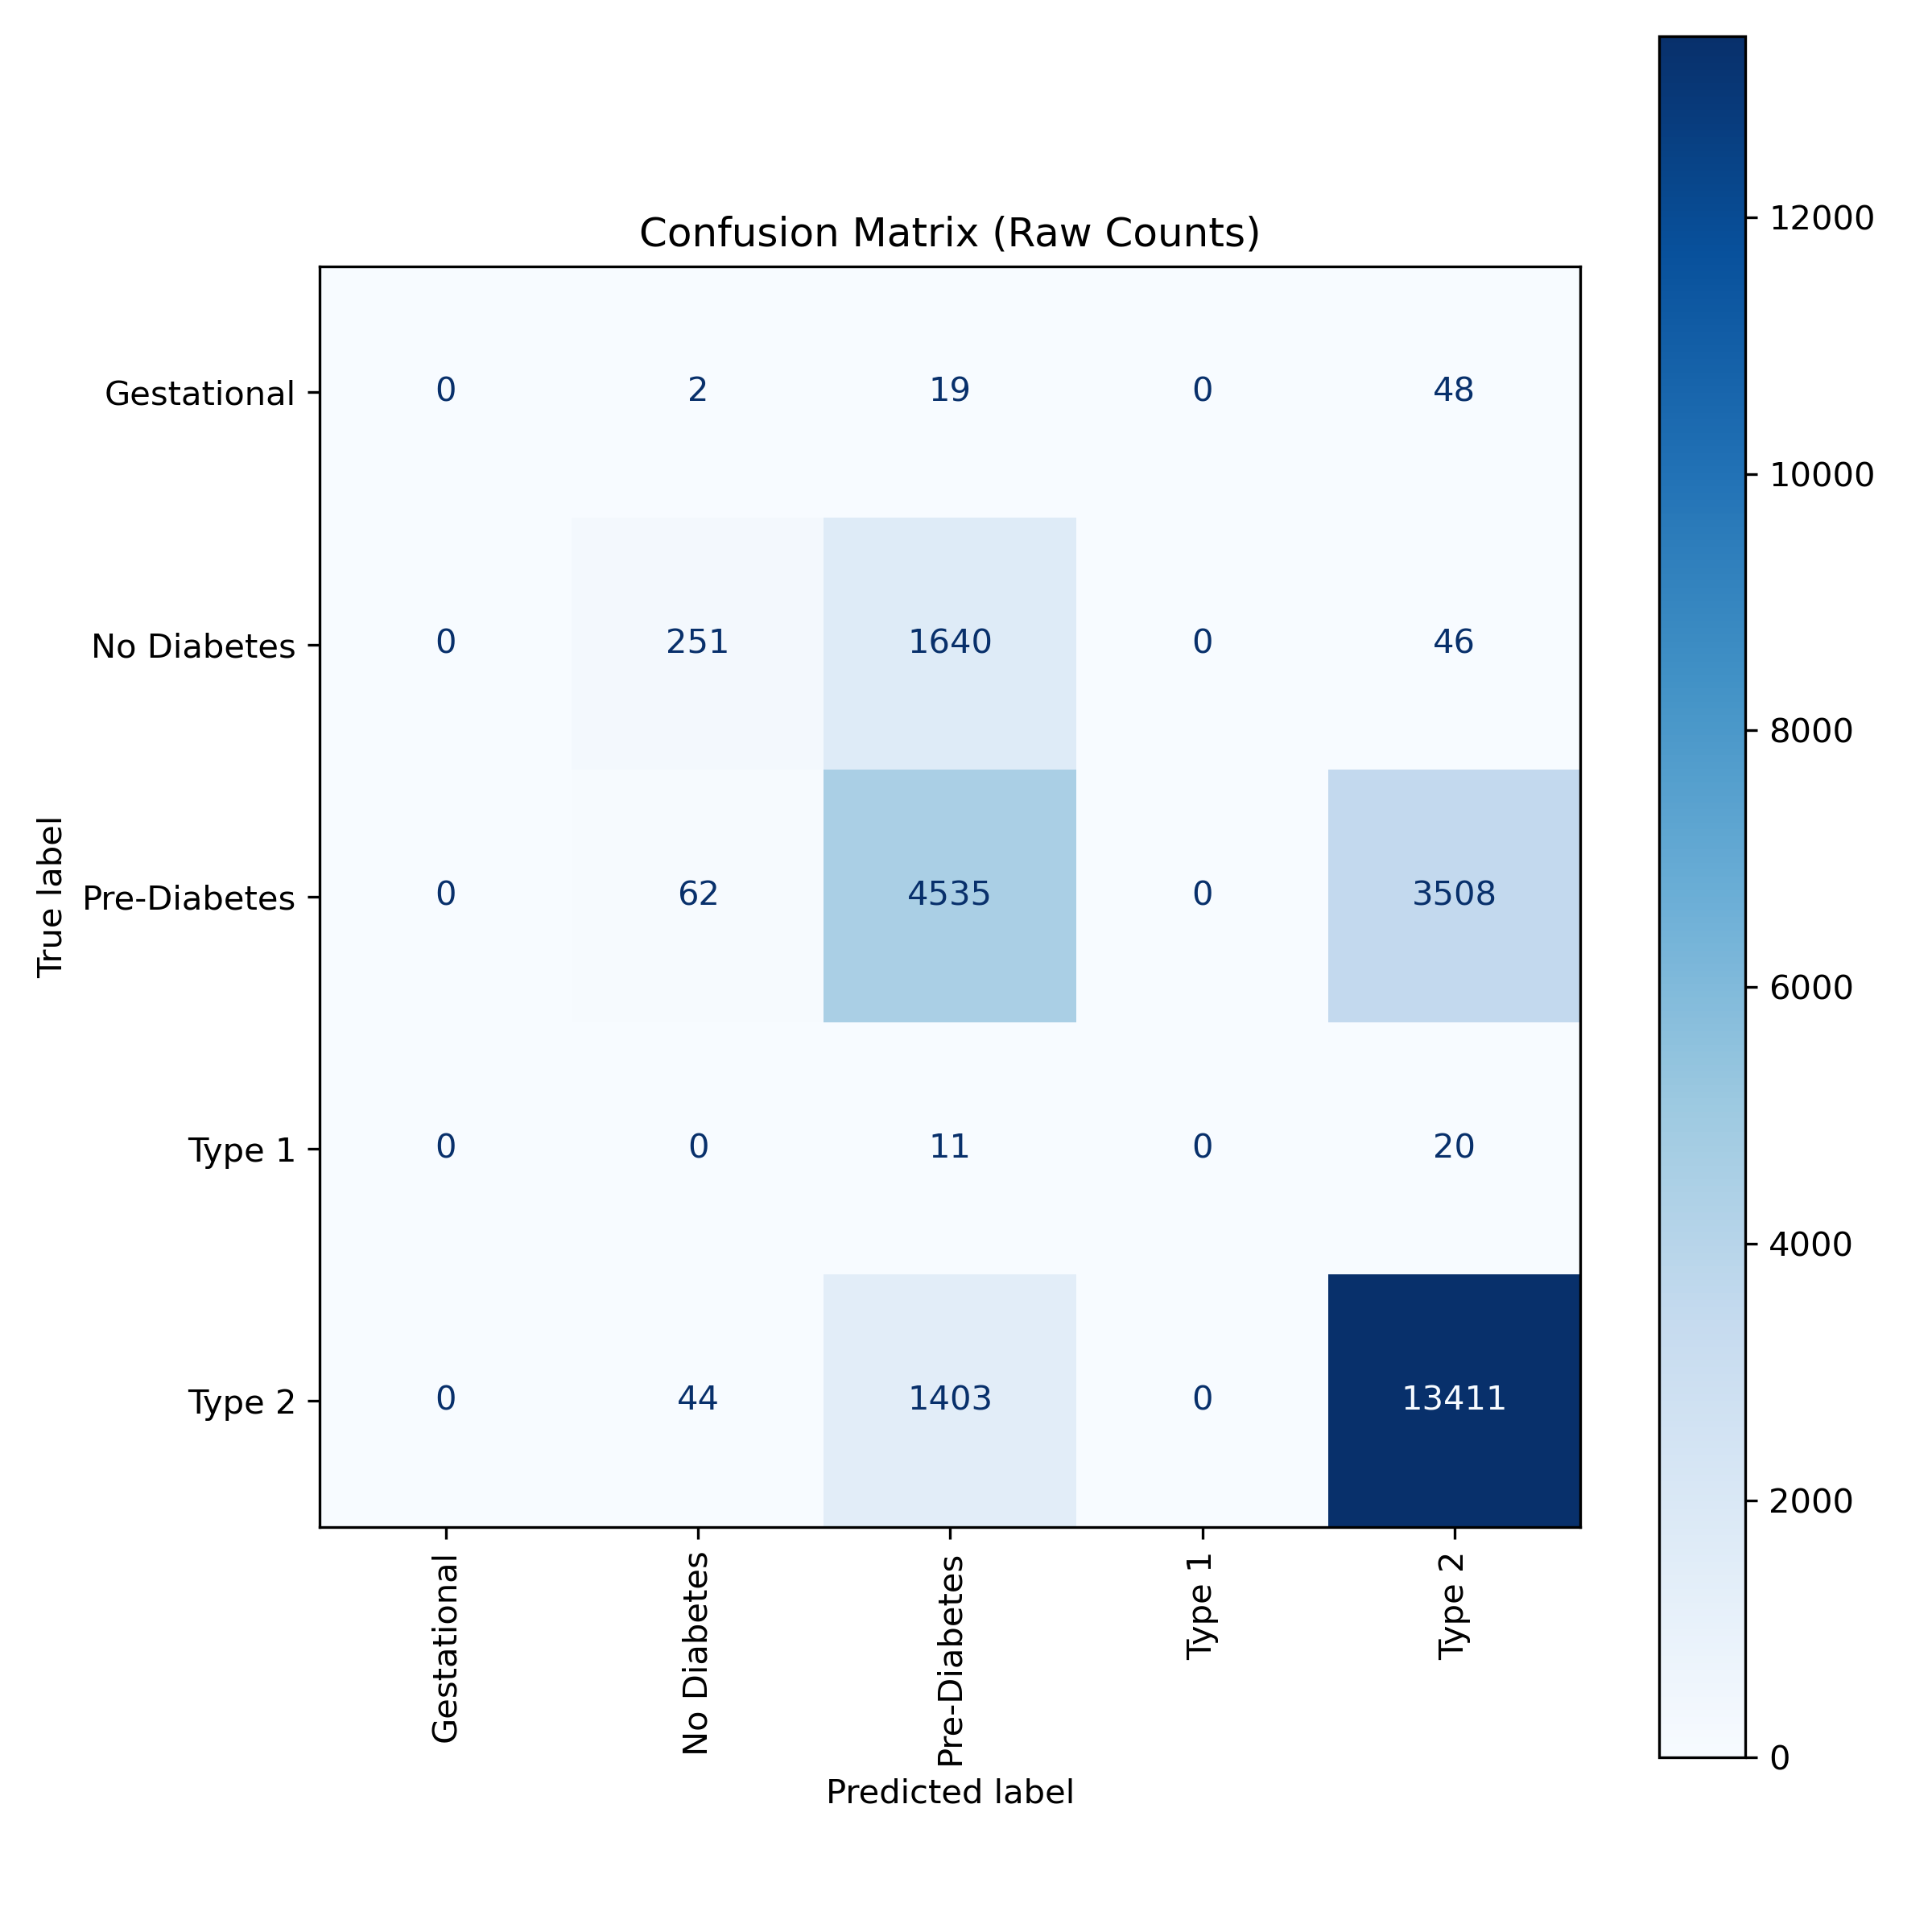
\includegraphics[scale=0.45]{log_ridge_confusion_matrix.png}}
	\caption{\textbf{Logistic/$\text{L}_2$ } Confusion Matrix}
	\label{ridge_confusion_matrix}
\end{figure}

\subsubsection{Logistic/$\text{L}_2$ Confusion Matrix} \indent The model demonstrates exceptional accuracy in identifying \textbf{Type 2 diabetes}, correctly classifying $\mathbf{13,411}$ out of $\mathbf{14,858}$ true cases as shown in Figure \ref{ridge_confusion_matrix}. However, it struggles significantly with other categories due in part to severe class imbalance, with Type 2 ($\mathbf{14,858}$ samples) and Pre-Diabetes ($\mathbf{8,105}$ samples) being dominant, while Gestational ($\mathbf{69}$) and Type 1 ($\mathbf{31}$) have very few samples.This imbalance likely contributes to the model's inability to correctly classify Gestational and Type 1 diabetes, resulting in \textbf{zero correct predictions} for both.\\
\indent Furthermore, high misclassification rates are observed because the model has two major "attractors": it frequently misclassifies other true classes as \textbf{Pre-Diabetes}, notably $\mathbf{1,640}$ cases of No Diabetes and $\mathbf{1,403}$ cases of Type 2, and it also frequently misclassifies other true classes as \textbf{Type 2}, especially $\mathbf{3,508}$ cases of Pre-Diabetes.

\begin{figure}[htbp]
	\centerline{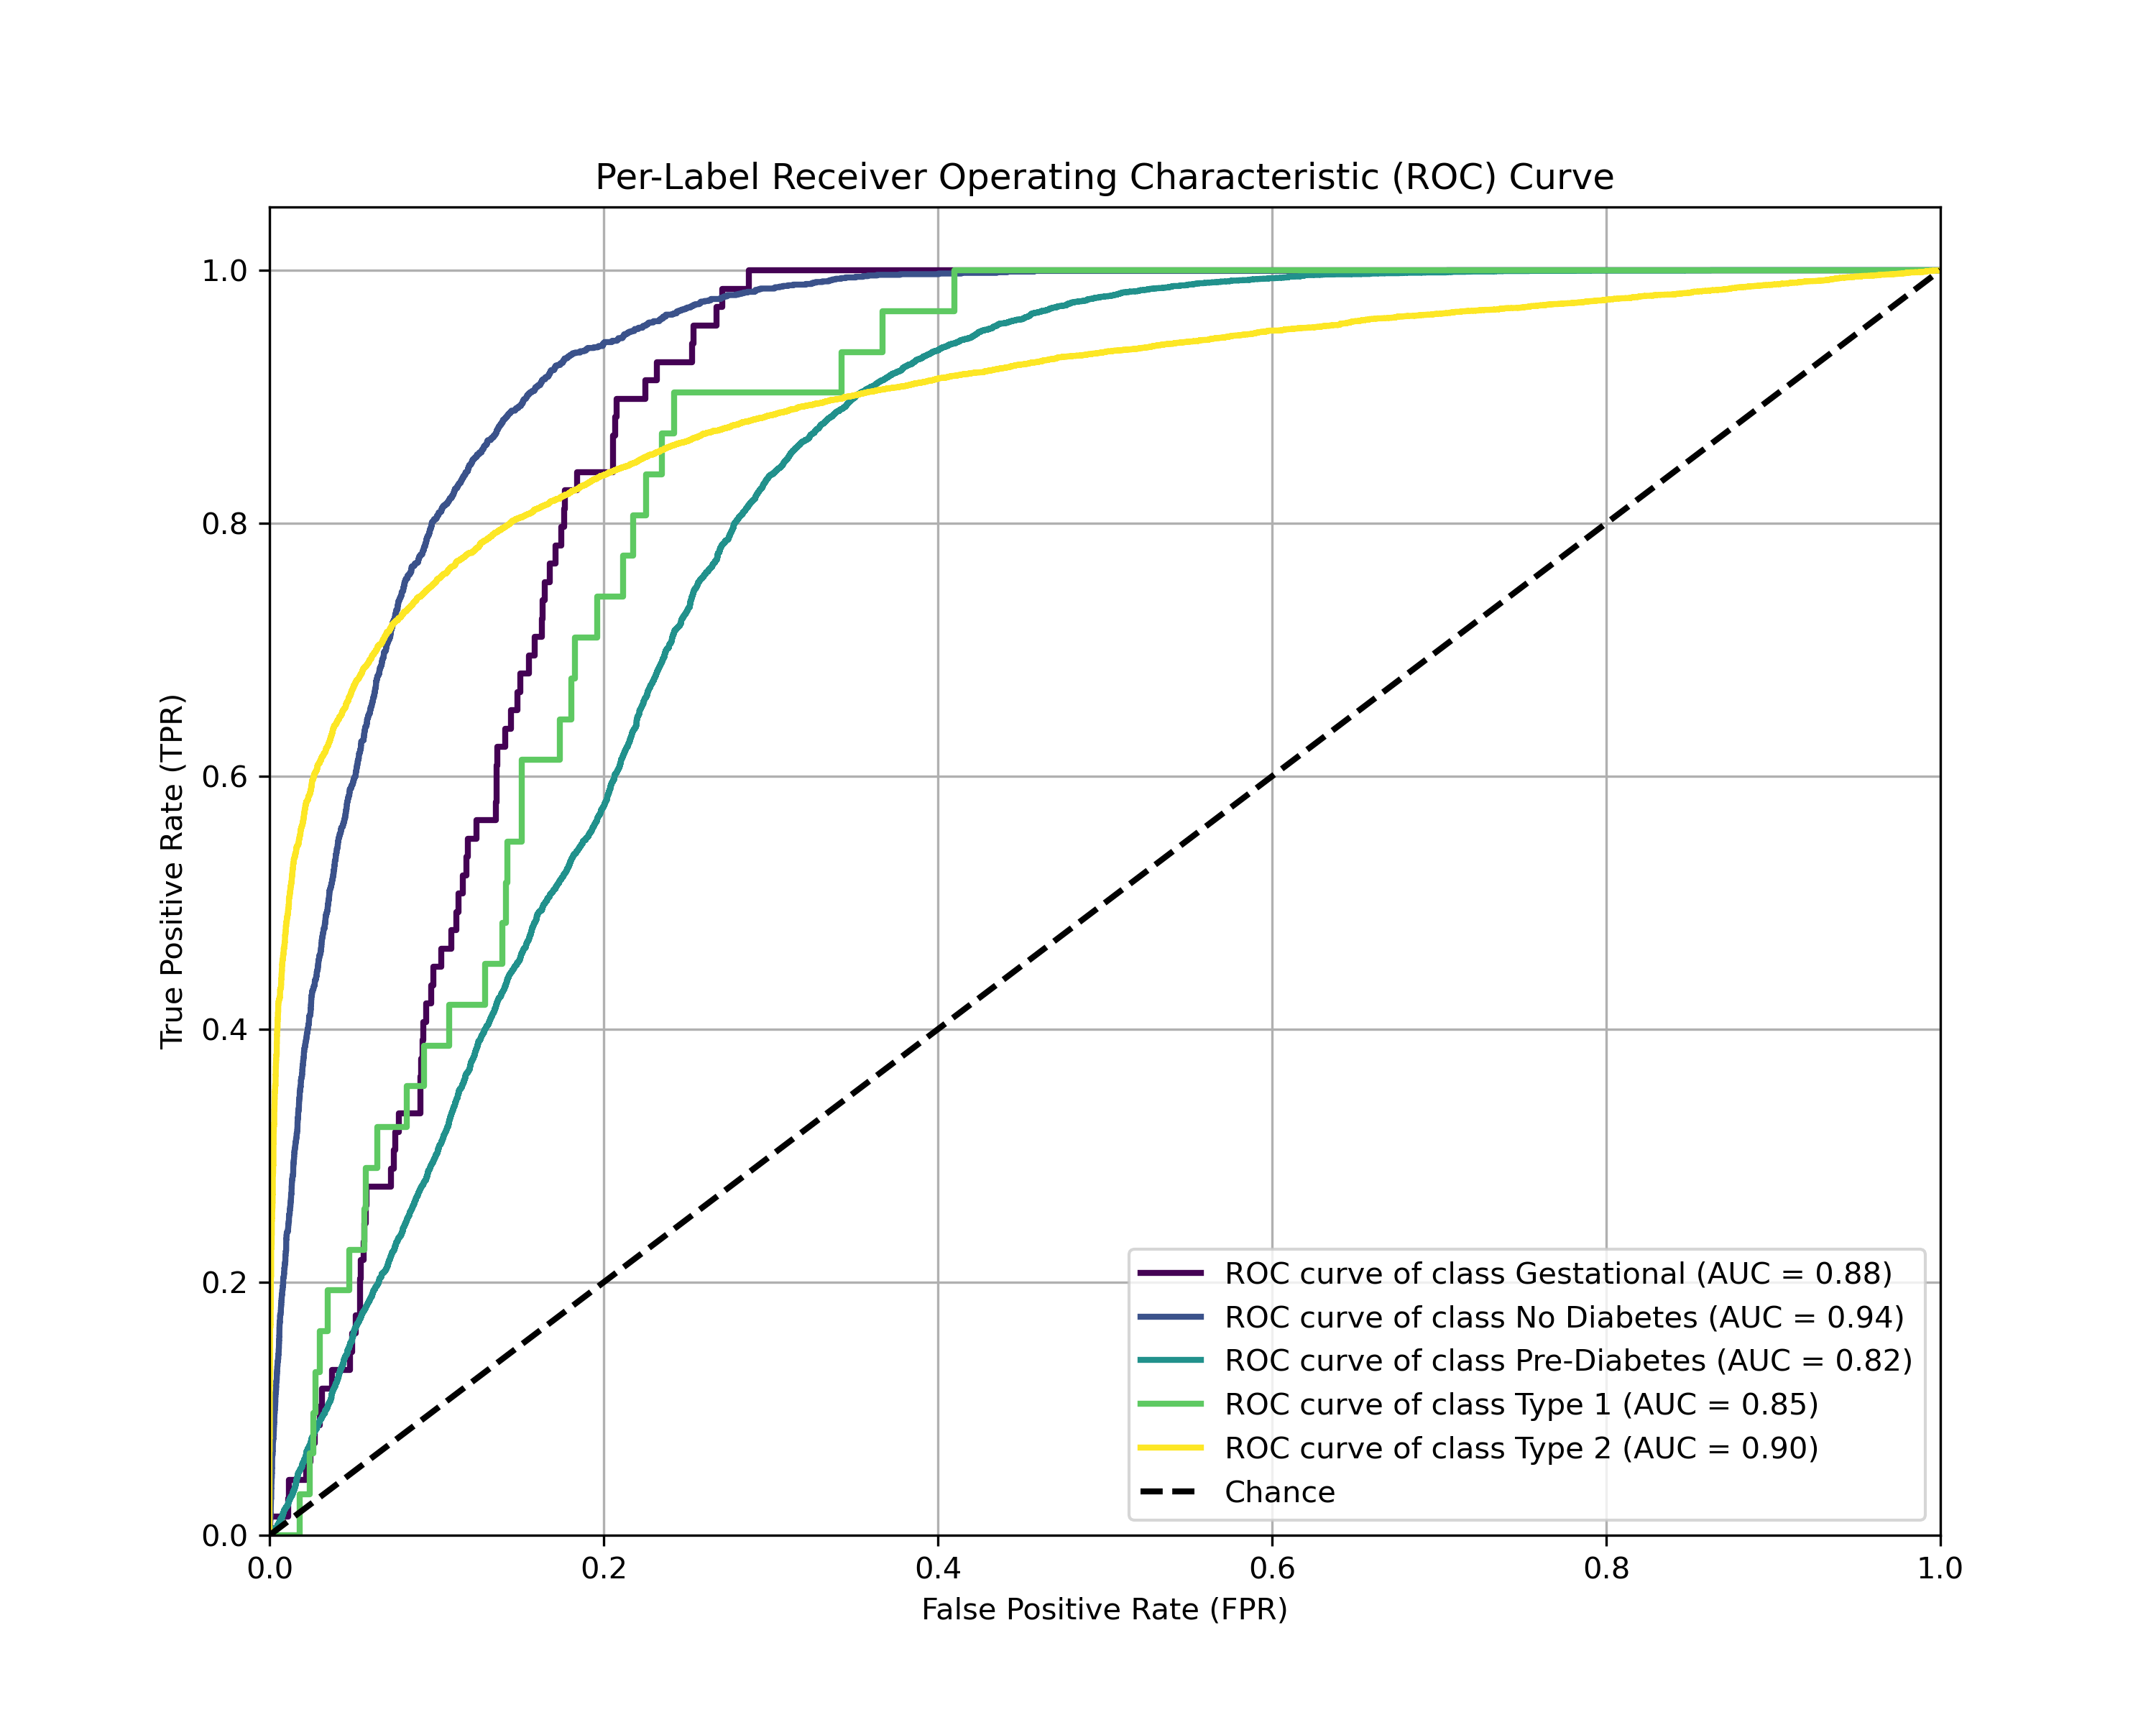
\includegraphics[scale=0.35]{log_ridge_roc_curve.png}}
	\caption{\textbf{Logistic/$\text{L}_2$ } ROC Curve}
	\label{ridge_roc_curve}
\end{figure}

\subsubsection{Logistic/$\text{L}_2$ ROC Curve} In Figure \ref{ridge_roc_curve} The classification model demonstrated varied but generally strong performance across the five categories. The \textbf{No Diabetes} class (Dark Blue curve, $\text{AUC} = 0.94$) showed the highest performance, indicating the model is excellent at distinguishing this group from the others. Following closely, the \textbf{Type 2} class (Yellow curve, $\text{AUC} = 0.90$) also exhibited very good performance.\\
\indent The classification of \textbf{Gestational} diabetes (Purple curve, $\text{AUC} = 0.88$) and \textbf{Type 1} diabetes (Light Green curve, $\text{AUC} = 0.85$) both showed good, solid performance. The class the model had the most difficulty distinguishing was \textbf{Pre-Diabetes} (Green/Teal curve, $\text{AUC} = 0.82$), which, although still a strong $\text{AUC}$ value, was the lowest among the five classes.\\

\subsection{\textbf{Logistic Regression with  ElasticNet Results}}

\subsubsection{Logistic/ElasticNet Confusion Matrix} The model's classification performance shows significant variance across the classes: the interpretation for \textbf{Gestational diabetes} is \textbf{Very Poor}, as the model failed to correctly identify any cases, with the majority being classified as Type 2; similarly, for \textbf{Type 1} diabetes, performance is \textbf{Very Poor} because the model identified zero true cases, shown in Figure \ref{elasticnet_confusion_matrix}. 

\begin{figure}[htbp]
	\centerline{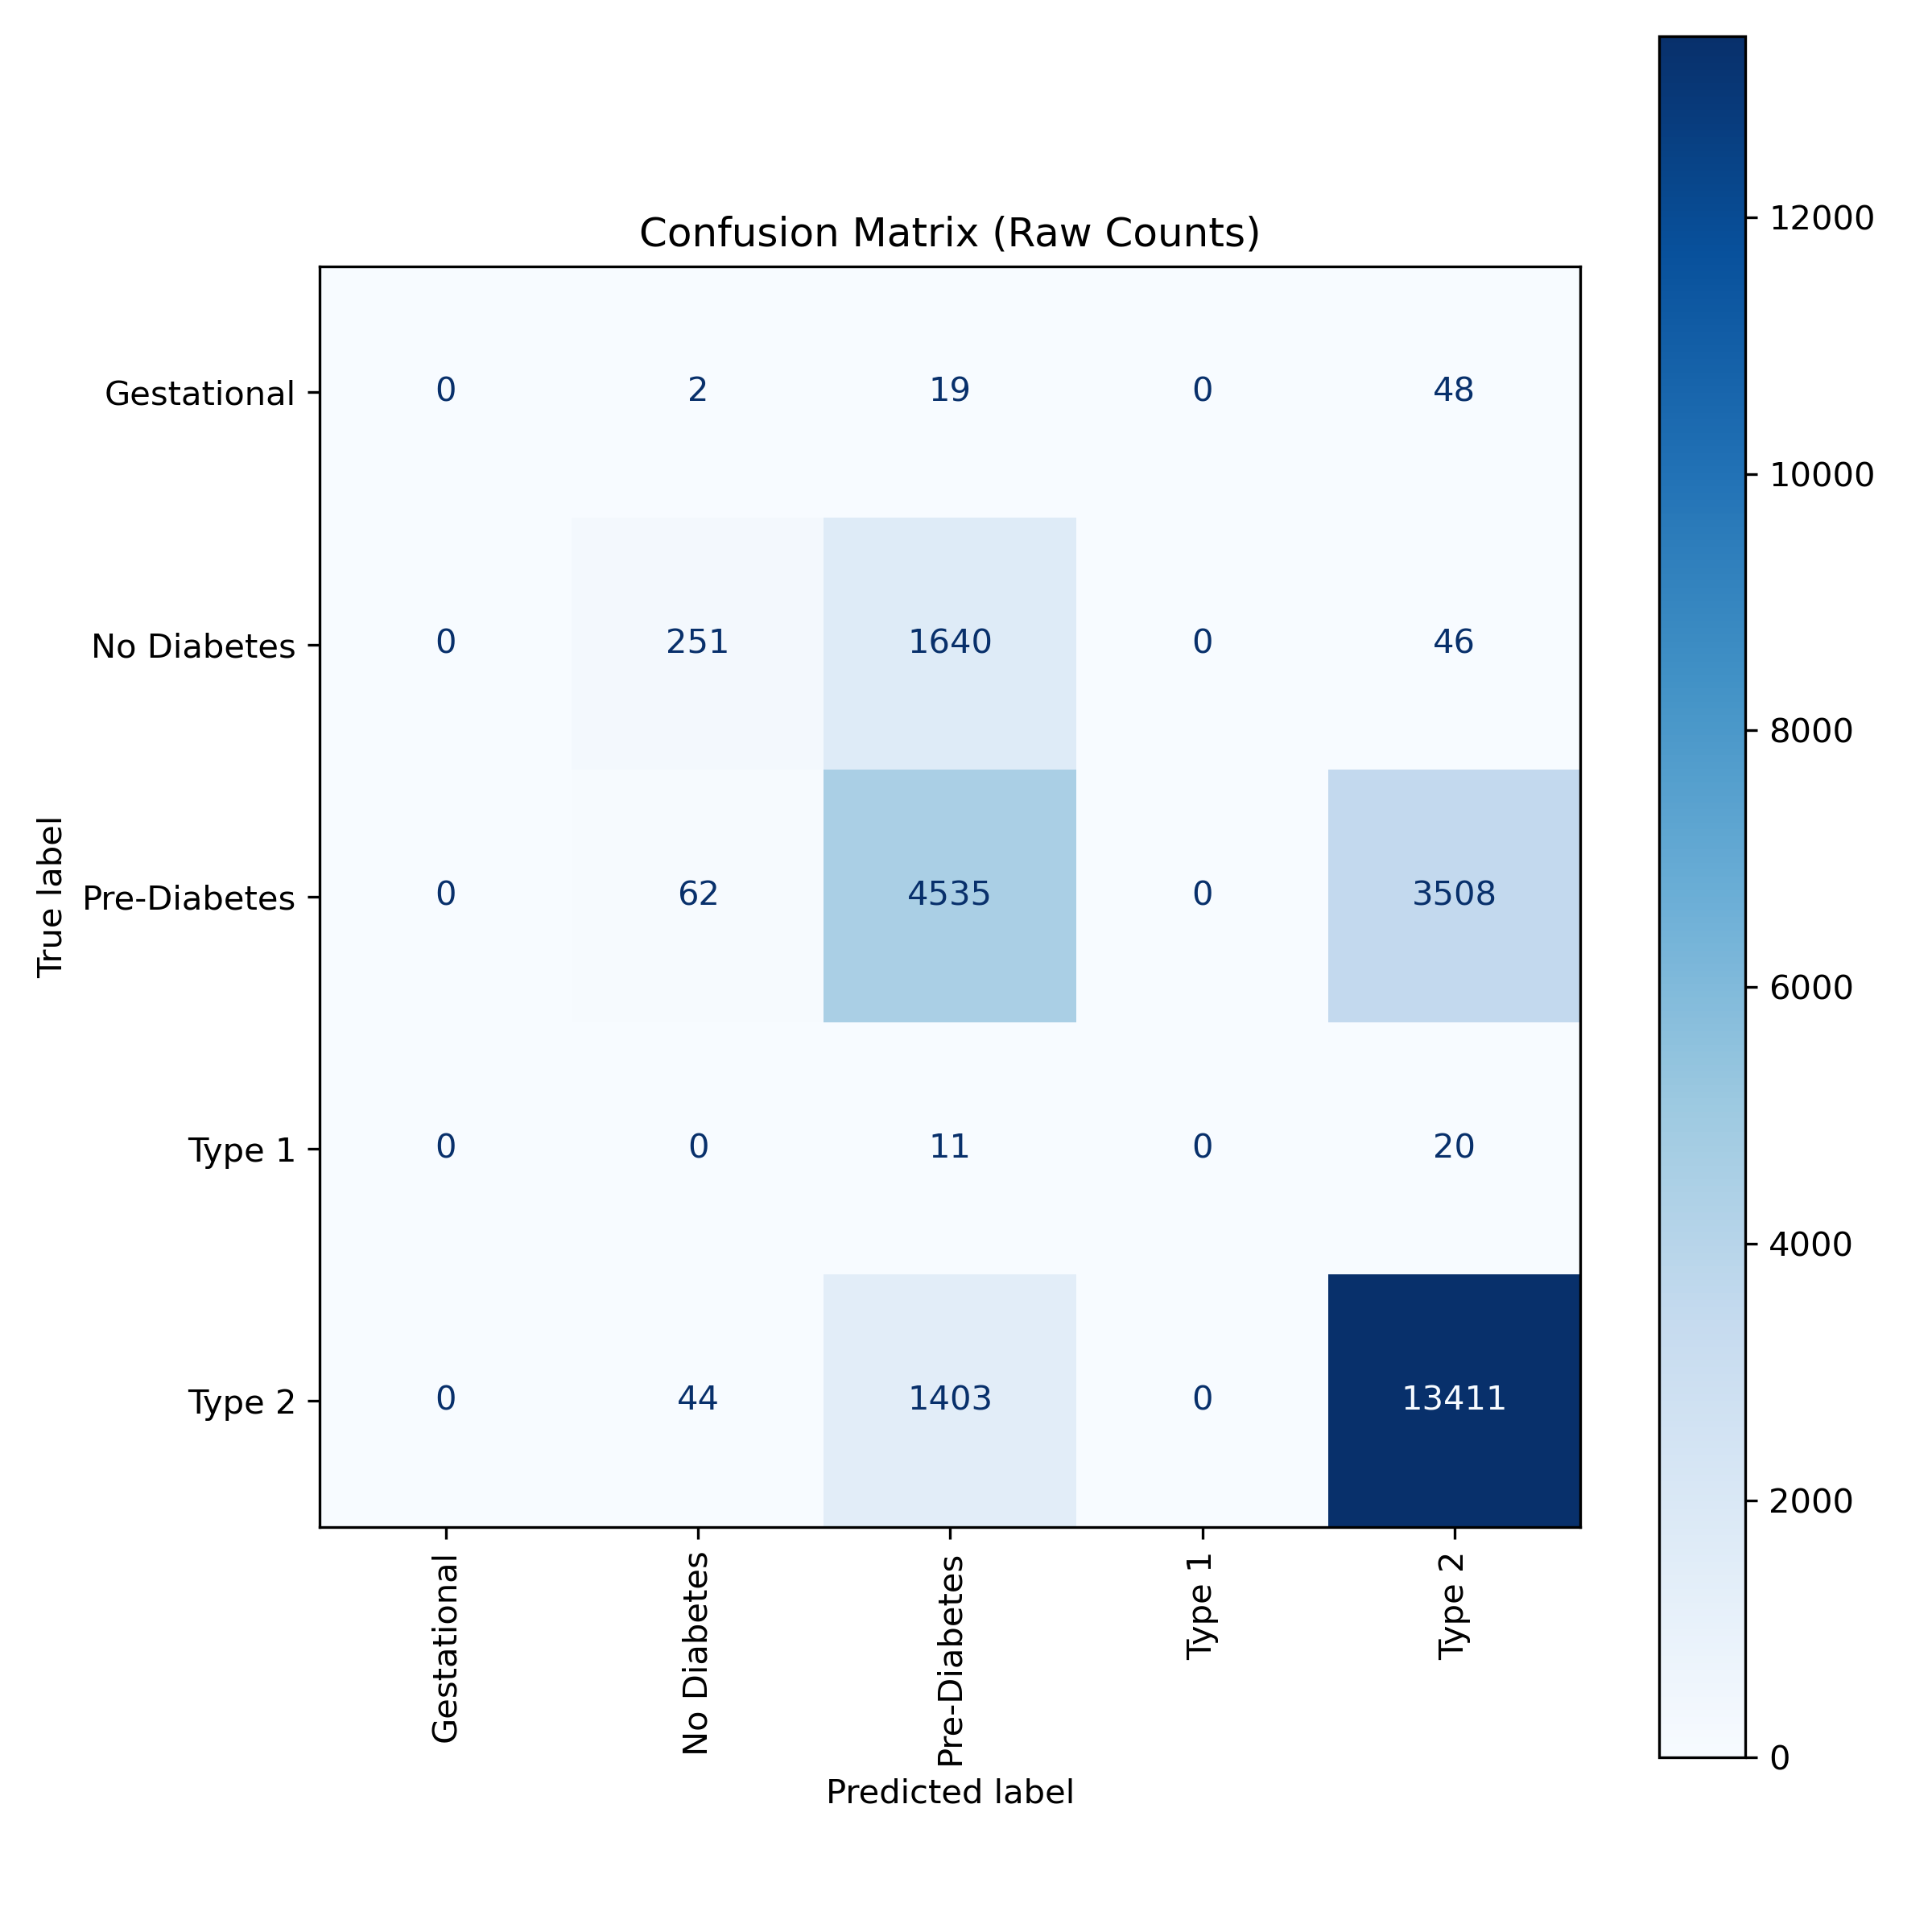
\includegraphics[scale=0.45]{log_elasticnet_confusion_matrix.png}}
	\caption{\textbf{Logistic/ElasticNet } Confusion Matrix}
	\label{elasticnet_confusion_matrix}
\end{figure}

\indent Performance for \textbf{No Diabetes} is \textbf{Poor}, as most true ``No Diabetes'' instances were incorrectly labeled as ``Pre-Diabetes'' (a significant false positive rate). The performance for \textbf{Pre-Diabetes} is \textbf{Moderate}, as the model correctly identified a large number, but a significant portion were misclassified as the more severe Type 2.\\
\indent Finally, for \textbf{Type 2} diabetes, the performance is \textbf{Strong}, indicating the model is highly accurate at identifying true Type 2 cases.

\begin{figure}[htbp]
	\centerline{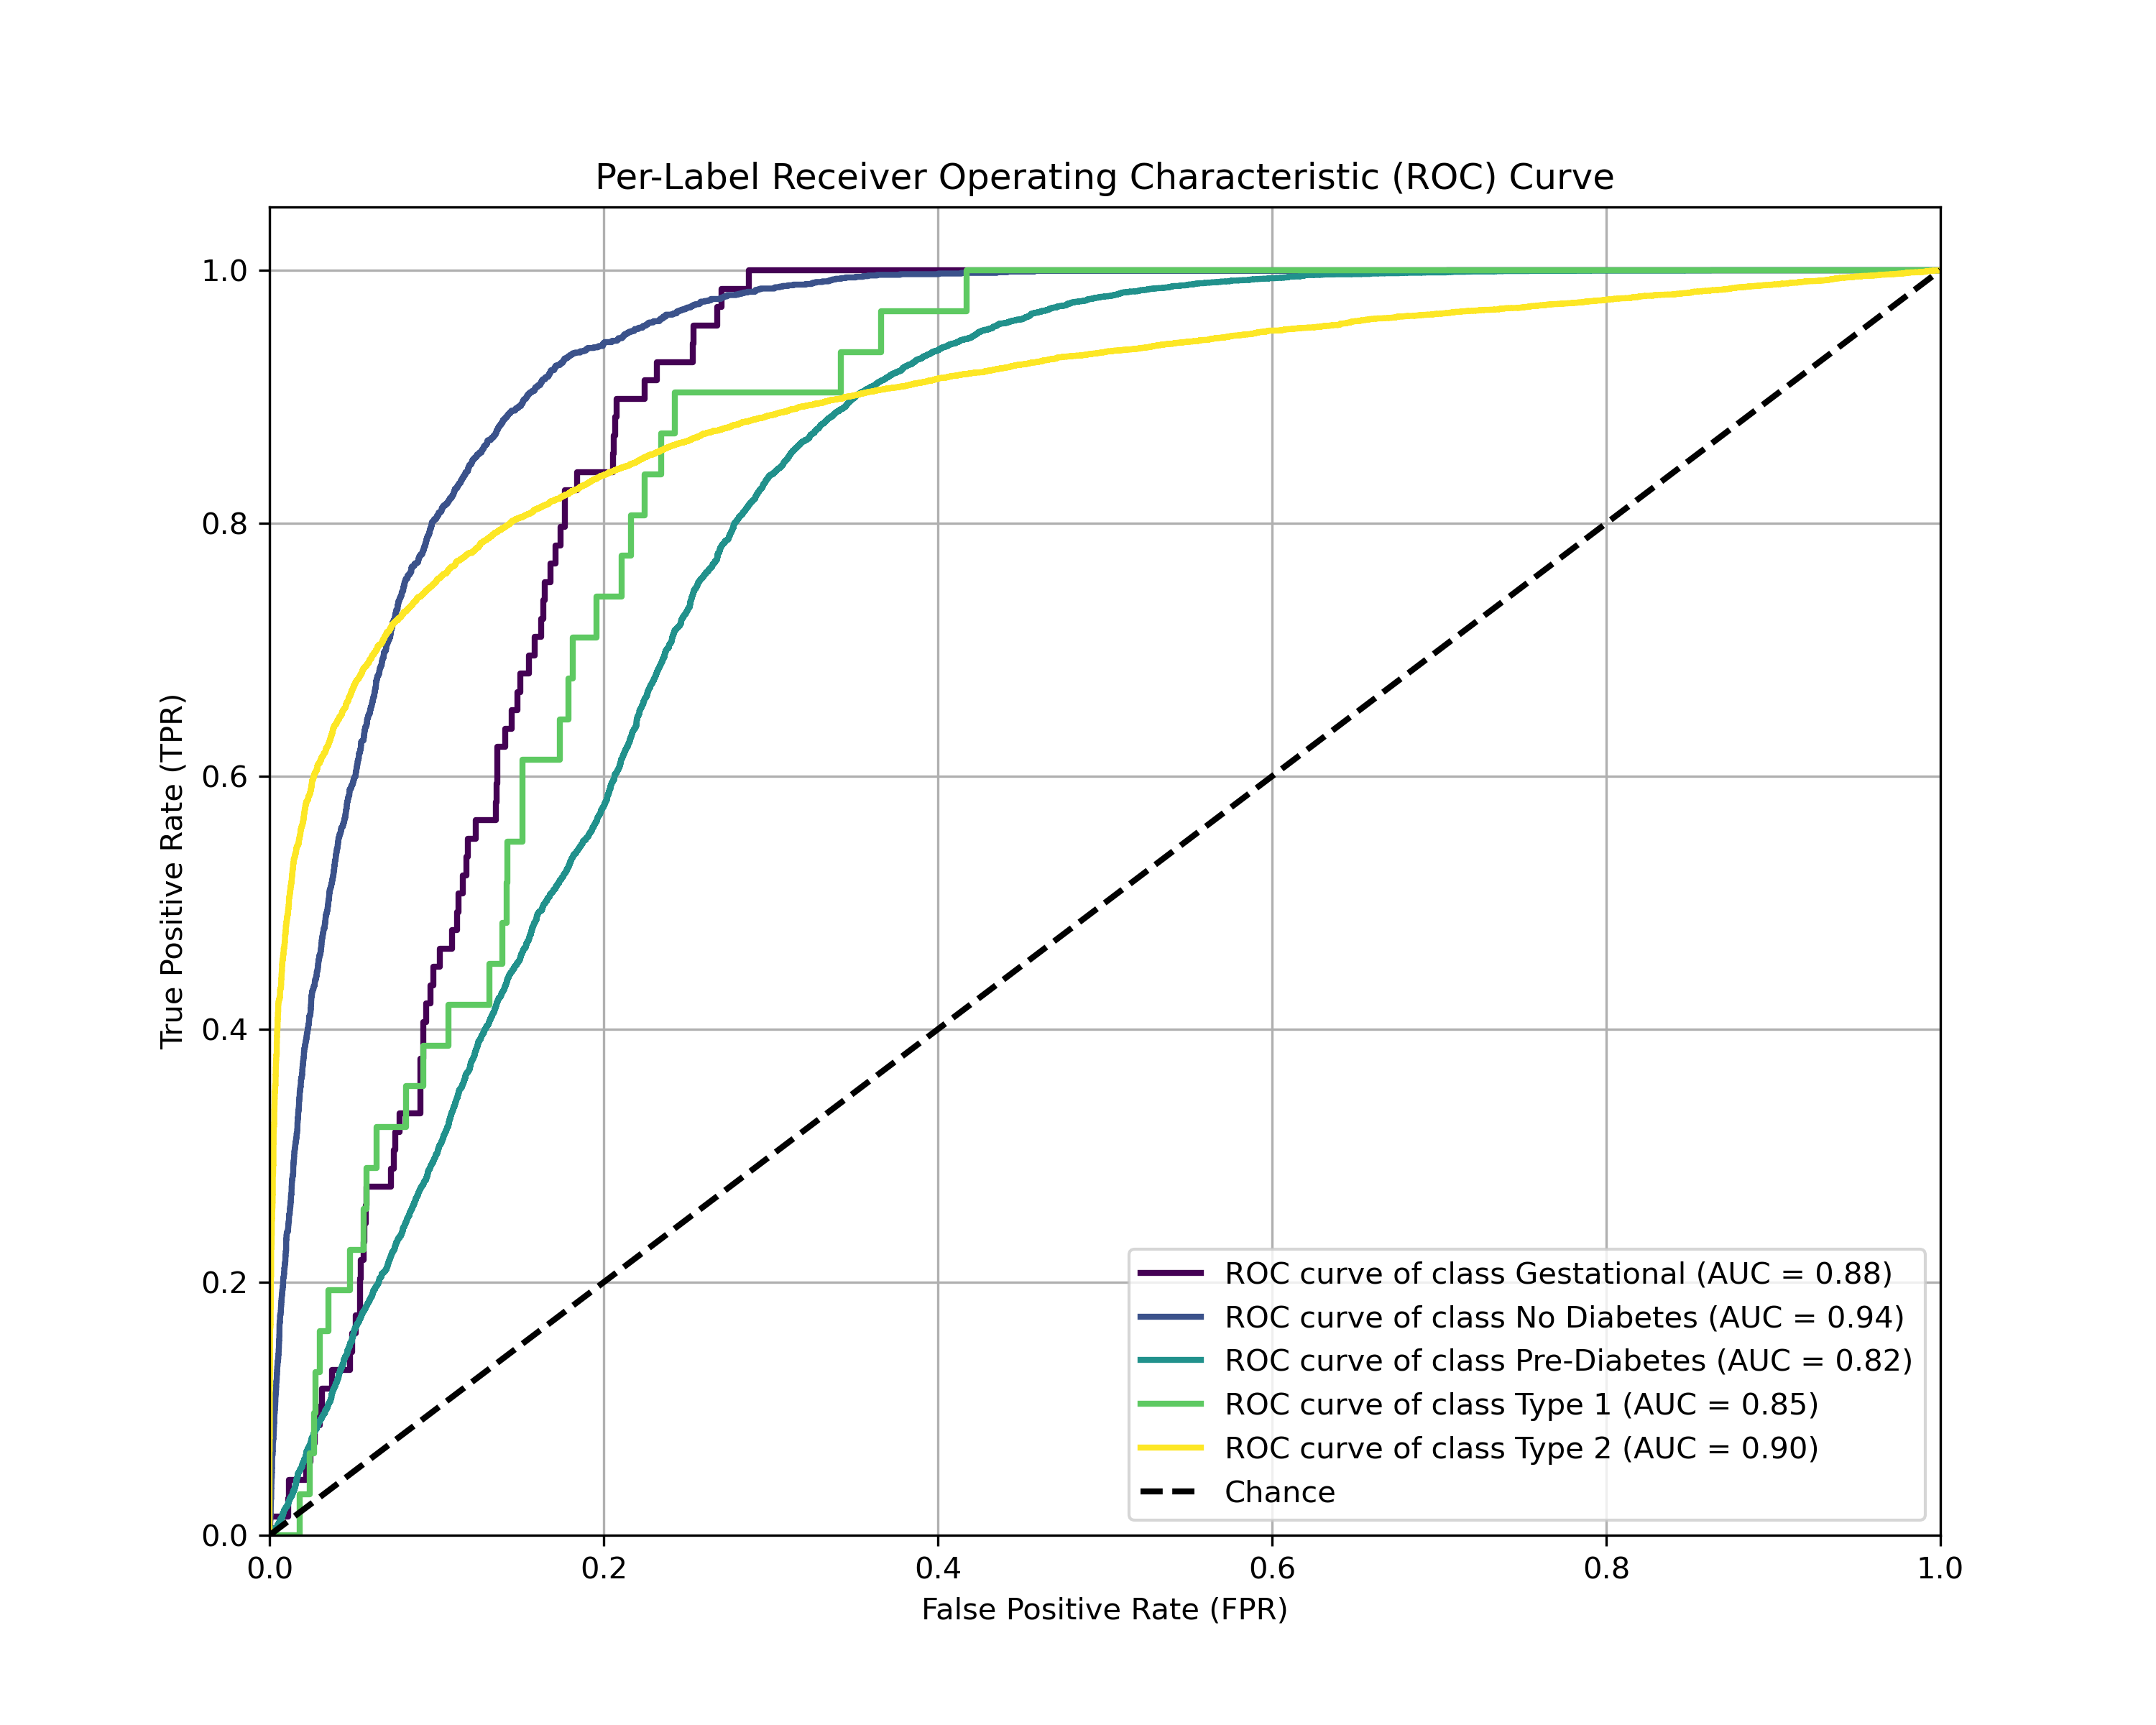
\includegraphics[scale=0.35]{log_elasticnet_roc_curve.png}}
	\caption{\textbf{Logistic/ElasticNet } ROC Curve}
	\label{elasticnet_roc_curve}
\end{figure}

\subsubsection{Logistic/ElasticNet ROC Curve} Figure \ref{elasticnet_roc_curve} evaluates the performance of a multi-class classification model, likely a \textbf{Logistic Regression} with \textbf{Elastic Net} regularization, across five distinct diabetes status classes by calculating the \textbf{Area Under the Curve (AUC)} for each class in a \textbf{one-vs-rest} manner. Identical to Figure \ref{ridge_roc_curve}.\\
\indent Overall, the model demonstrates strong diagnostic capability, with all classes yielding AUC values significantly above the $0.50$ chance level. Specifically, the model performs \textbf{excellently} in identifying the \textbf{No Diabetes} class ($\text{AUC} = 0.94$), followed closely by \textbf{Type 2} ($\text{AUC} = 0.90$) and \textbf{Gestational} ($\text{AUC} = 0.88$), indicating a very high effectiveness in separating these groups from the rest.\\
\indent The performance is still \textbf{good} for \textbf{Type 1} ($\text{AUC} = 0.85$), but the model shows its lowest performance for the \textbf{Pre-Diabetes} class ($\text{AUC} = 0.82$), suggesting this class presents the greatest classification difficulty compared to the others.

\section{\textbf{Discussion}}

\subsection{Models Performance}

\begin{table}[h!]
	\centering
	\caption{Performance Metrics: Logistic Regression ($\text{L}_1$ and $\text{L}_2$)}
	\label{tab:logreg_l1_l2_performance}
	\begin{tabular}{|l|c|c|}
		\hline
		\textbf{Metric} & \textbf{Logistic/$\text{L}_1$} & \textbf{Logistic/$\text{L}_2$} \\
		\hline
		\textbf{Best CV  $F_1$ Weighted} & 0.7139 & 0.6995 \\
		\hline
		\textbf{Test $F_1$ Weighted Score} & 0.7146 & 0.7039 \\
		\hline
		\textbf{Overall Test Accuracy} & 0.7398 & 0.7279 \\
		\hline
		\textbf{Overall Error Rate} & 0.2602 & 0.2721 \\
		\hline
	\end{tabular}
\end{table}

\begin{table}[h!]
	\centering
	\caption{Performance Metrics: Logistic/ElasticNet and KNN}
	\label{tab:elasticnet_knn_performance}
	\begin{tabular}{|l|c|c|}
		\hline
		\textbf{Metric} & \textbf{Logistic/ElasticNet} & \textbf{KNN} \\
		\hline
		\textbf{Best CV $F_1$ Weighted} & 0.6996 & 0.7475 \\
		\hline
		\textbf{Test $F_1$ Weighted Score} & 0.7039 & 0.7483 \\
		\hline
		\textbf{Overall Test Accuracy} & 0.7279 & 0.7492 \\
		\hline
		\textbf{Overall Error Rate} & 0.2721 & 0.2508 \\
		\hline
	\end{tabular}
\end{table}

\indent The \textbf{KNN} model is the superior performer, achieving the highest \textbf{Overall Test Accuracy} ($\mathbf{0.7492}$) and the lowest \textbf{Overall Error Rate} ($\mathbf{0.2508}$) on unseen data, as shown in Tables \ref{tab:logreg_l1_l2_performance} and \ref{tab:elasticnet_knn_performance}. Its \textbf{Test $F_1$ Weighted Score} is also the highest, and its close \textbf{CV $F_1$ Weighted Score} score suggests effective generalization.\\
\indent The closeness between its Best Cross-Validation ($\text{CV}$) $F_1$ score ($\mathbf{0.7475}$) and Test $F_1$ score ($\mathbf{0.7483}$) suggests that the model is well-tuned and avoiding significant overfitting.\\
\indent The multi-class classification models---including \textbf{KNN}, and \textbf{Logistic/$\text{L}_1$}, \textbf{Logistic/$\text{L}_2$}, and \textbf{Logistic/ElasticNet} regularization---all exhibit a common and significant challenge: a systematic bias toward the most prevalent classes, \textbf{Type 2 Diabetes} and \textbf{Pre-Diabetes}, resulting in poor performance on minority classes.\\
\indent This results in poor performance, particularly for minority classes like Gestational and Type 1 Diabetes. Specifically, \textbf{KNN} completely fails to classify Gestational and Type 1 Diabetes, while the \textbf{Logistic/$\text{L}_1$} model is the worst, functioning as a poor binary classifier with zero accuracy for three classes due to aggressive feature elimination.

\subsection{Features Importance}

\subsubsection{The Difference between Logistic/$\text{L}_2$ and Logistic/ElasticNet}

\indent The tables \ref{tab:ridge_positive_coefficients}, \ref{tab:elasticnet_positive_coefficients}, \ref{tab:ridge_negative_coefficients} and \ref{tab:ridge_negative_coefficients} of the \textbf{Logistic/$\text{L}_2$} and \textbf{Logistic/ElasticNet} models consistently shows that being female is the strongest positive predictor for \textbf{Gestational diabetes}, while high postprandial glucose is the most significant positive predictor for \textbf{Type 2 diabetes}.\\
\indent Conversely, being male serves as a strong negative predictor (or a strong argument against) a Gestational diabetes diagnosis, and high postprandial glucose is a powerful indicator against classification in the \textbf{No Diabetes} group.\\
\indent The agreement between both regularization models on the direction and magnitude of these key features confirms that these predictive relationships are robust and reliable.\\
\indent Both models showed identical AUC, ROC, and metrics, attributable to ElasticNet tuning to $66\%$ $\text{L}_2$ regularization.\\

\begin{table}[h!]\centering
	\caption{Top 10 Positive Coefficients for Logistic/$\text{L}_2$  Model}
	\label{tab:ridge_positive_coefficients}
	\begin{tabular}{|c|c|c|c|}
		\hline
		\textbf{Rank} & \textbf{Feature} & \textbf{Class} & \textbf{Value} \\
		\hline
		1 & gender\_Female & Gestational & 2.5781 \\
		2 & glucose\_postprandial & Type 2 & 2.2145 \\
		3 & family\_history\_diabetes & Type 2 & 0.7400 \\
		4 & physical\_activity\_minutes\_per\_week & No Diabetes & 0.2506 \\
		5 & age & Type 2 & 0.2187 \\
		6 & hdl\_cholesterol & Type 1 & 0.2048 \\
		7 & gender\_Other & Type 2 & 0.2034 \\
		8 & hypertension\_history & Type 1 & 0.1936 \\
		9 & ldl\_cholesterol & Type 1 & 0.1369 \\
		10 & glucose\_postprandial & Gestational & 0.1194 \\
		\hline
	\end{tabular}
\end{table}

\begin{table}[h!]\centering
	\caption{Top 10 Positive Coefficients for Logistic/ElasticNet Model}
	\label{tab:elasticnet_positive_coefficients}
	\begin{tabular}{|c|c|c|c|}
		\hline
		\textbf{Rank} & \textbf{Feature} & \textbf{Class} & \textbf{Value} \\
		\hline
		1 & gender\_Female & Gestational & 3.7099 \\
		2 & glucose\_postprandial & Type 2 & 2.2146 \\
		3 & family\_history\_diabetes & Type 2 & 0.7402 \\
		4 & physical\_activity\_minutes\_per\_week & No Diabetes & 0.2505 \\
		5 & age & Type 2 & 0.2186 \\
		6 & hdl\_cholesterol & Type 1 & 0.2055 \\
		7 & gender\_Other & Type 2 & 0.2037 \\
		8 & hypertension\_history & Type 1 & 0.1982 \\
		9 & ldl\_cholesterol & Type 1 & 0.1386 \\
		10 & glucose\_postprandial & Gestational & 0.1195 \\
		\hline
	\end{tabular}
\end{table}

\begin{table}[h!]\centering
	\caption{Top 10 Negative Coefficients for Logistic/$\text{L}_2$ Model}
	\label{tab:ridge_negative_coefficients}
	\begin{tabular}{|c|c|c|c|}
		\hline
		\textbf{Rank} & \textbf{Feature} & \textbf{Class} & \textbf{Value} \\
		\hline
		1 & gender\_Male & Gestational & -4.3410 \\
		2 & glucose\_postprandial & No Diabetes & -2.4411 \\
		3 & gender\_Other & Gestational & -1.9866 \\
		4 & employment\_status\_Student & Type 1 & -1.6044 \\
		5 & family\_history\_diabetes & No Diabetes & -1.4740 \\
		6 & age & Type 1 & -1.4634 \\
		7 & smoking\_status\_Former & Gestational & -1.3612 \\
		8 & employment\_status\_Retired & Gestational & -1.3124 \\
		9 & gender\_Female & Type 1 & -1.2712 \\
		10 & smoking\_status\_Never & Gestational & -1.2301 \\
		\hline
	\end{tabular}
\end{table}

\begin{table}[h!]\centering
	\caption{Top 10 Negative Coefficients for Logistic/ElasticNet Model}
	\label{tab:elasticnet_negative_coefficients}
	\begin{tabular}{|c|c|c|c|}
		\hline
		\textbf{Rank} & \textbf{Feature} & \textbf{Class} & \textbf{Value} \\
		\hline
		1 & gender\_Male & Gestational & -5.4887 \\
		2 & gender\_Other & Gestational & -2.4660 \\
		3 & glucose\_postprandial & No Diabetes & -2.4413 \\
		4 & employment\_status\_Student & Type 1 & -1.6300 \\
		5 & smoking\_status\_Former & Gestational & -1.5230 \\
		6 & family\_history\_diabetes & No Diabetes & -1.4744 \\
		7 & age & Type 1 & -1.4689 \\
		8 & employment\_status\_Retired & Gestational & -1.4324 \\
		9 & smoking\_status\_Never & Gestational & -1.3907 \\
		10 & smoking\_status\_Current & Gestational & -1.3193 \\
		\hline
	\end{tabular}
\end{table}

\subsubsection{Glucose Postprandial Dominance}
The \texttt{glucose\_postprandial} feature was universally dominant across all models. While \textbf{Logistic/$\text{L}_2$} and \textbf{Logistic/ElasticNet} provided a more detailed view of its application, both \textbf{KNN} and \textbf{Logistic/$\text{L}_1$} also utilized it extensively, with \textbf{Logistic/$\text{L}_1$} relying on it as the sole feature for its predictions due to its aggressive feature selection.


\section{\textbf{Conclusion(s)}}

\indent Despite testing various models (\textbf{Logistic Regression} with LASSO, ElasticNet, and Ridge regularization, and \textbf{$K$-Nearest Neighbors (KNN)}) on this complex, imbalanced multiclass dataset \cite{rakesh_kolipaka_ranjith_kumar_digutla_2025}, none of the models demonstrated sufficient robustness, as they consistently failed to accurately classify the least frequently observed classes, specifically Gestational and Type 1 stage diabetes.\\
\indent \textbf{The overall performance for all models was poor, with approximately one out of every four classifications being incorrect}.\\
\indent While Logistic Regression like \textbf{Logistic/ElasticNet} and \textbf{Logistic/$\text{L}_2$} yielded superior \textbf{AUC} scores (indicating better discriminatory power), the best overall test accuracy was achieved by \textbf{KNN} ($\mathbf{0.7492}$), closely followed by \textbf{Logistic/$\text{L}_1$} ($\mathbf{0.7398}$), a finding consistent with the weighted $F_1$ metric.\\
\indent The feature \texttt{glucose\_postprandial} was identified as the most effective single predictor across all models for classification.\\
\indent Based solely on the performance metrics presented, \textbf{the KNN model is the most recommendable choice} as its superior accuracy and weighted $F_1$ score outweigh the higher interpretability offered by the Logistic Regression models. Suggesting it has the best performance in the final classification task.

\section*{\textbf{Appendix}}
	
\section*{Appendix A: Supplementary Materials and Software Usage}
\subsection*{Source Code Repository \label{app:code}}
The source code, data, and detailed implementation scripts for this project are available on GitHub \\
(URL:\texttt{ https://github.com/}
\texttt{gaguillen4384-dev/Data-Science/} \\
\texttt{/DataMining\_1/Project\_3}).
\\
\subsection*{Software Usage Acknowledgment}
The text and documentation were edited and refined using Google Gemini.

\begin{thebibliography}{9} % '9' is for formatting the numbering (up to 9 items)
	
\bibitem{rakesh_kolipaka_ranjith_kumar_digutla_2025}
Kolipaka, Rakesh, \& Digutla, Ranjith Kumar. (2025). \textbf{Diabetes Health Indicators Dataset}. 
Kaggle. Available at: \texttt{https://www.kaggle.com/dsv/13128284}. 
DOI: \texttt{10.34740/KAGGLE/DSV/13128284}.
	
\end{thebibliography}

\vspace{12pt}

\end{document}
